
\documentclass{article}
\usepackage[utf8]{inputenc}
\usepackage[titletoc, title]{appendix}
\usepackage{geometry}
\geometry{
 a4paper,
 left=27mm,
 top=30mm,
 }
\usepackage{ amssymb }
\usepackage{graphicx} % Required for the inclusion of images
\usepackage{caption}
\usepackage{subcaption}
\usepackage{amsmath} % Required for some math elements
\usepackage[labelfont=bf]{caption}



\usepackage{hyperref}
\usepackage{float}






%\setlength\parindent{0pt} % Removes all indentation from paragraphs
\usepackage{authblk}
\usepackage{wrapfig}
%\renewcommand{\labelenumi}{\alph{enumi}.} % Make numbering in the enumerate environment by letter rather than number (e.g. section 6)
\usepackage[font={small}]{caption}
%\newcommand*\diff{\mathop{}\!\mathrm{d}}
\usepackage{tikz}
\usepackage{placeins}



%----------------------------------------------------------------------------------------
%	DOCUMENT INFORMATION
%----------------------------------------------------------------------------------------

\title{QUANTITATIVE MODELS OF BEHAVIOR} % Title

\author{Florian \textsc{Leprévost}} % Author name

\date{\today} % Date for the report

\begin{document}
\maketitle % Insert the title, author and date
\tableofcontents

\begin{center}
\begin{tabular}{l r}
Supervisor: Manuel Beiran % Instructor/supervisor
\end{tabular}
\end{center}


\section{Introduction}

\indent\indent Experimental psychology and neuroscience have uncovered many rules underlying behavior over the years, which have been used to create computational models.  Modeling behavior can be useful for several reasons, for instance to hypothesize on the computations made in the brain and see if it ``fits" the data; or to use those findings to create better performing learning algorithms.
%----------------------------------------------------------------------------------------
%	SECTION 1
%----------------------------------------------------------------------------------------

\section{Reinforcement learning}
\indent\indent Probably the most notable and described behavior is the learning mechanisms underlying Pavlov's conditioning experiments. The simplest way to understand classical conditioning, is that an agent automatically associates a reward or conditioned stimulus (CS; \textit{e.g.} food) with a state of the environment or unconditionned stimulus (US), not naturally relevant to the agent (\textit{e.g.} a bell). After some learning, the US is enough to elicitates a response (\textit{e.g.} salivary) in the agent: one can then imagine that there is an internal estimate of what the US yields, \textit{i.e.} the agent predicts the apparition of a reward.
\\
\indent Considering this, some have proposed a model where the internal estimate $w$ is updated following a simple rule depending on the prediction error $\delta$: the Rescorla-Wagner rule or delta-rule.
A simple implementation of it can be the following. Let $u$ be the US, $r$ be the actual reward, and $v$ is the predicted reward, such that:


\begin{align*}
  \bigg\{
      &\begin{array}{ll}
          u=0  \;\;\; \mbox{if US absent}\\
          u=1  \;\;\; \mbox{if US present}
      \end{array}
  &&\bigg\{
      \begin{array}{ll}
          r=0  \;\;\; \mbox{if CS absent}\\
          r=1  \;\;\; \mbox{if CS present}
      \end{array}
  \\
  \\
  &\delta = r-v
   &&v= wu
  \intertext{And the Rescorla-Wagner rule propose to update $w$ as follows:}
  &w \leftarrow w + \epsilon \delta u
  \;\;\;\;\;\;\;\;\;\;
   &&\text{with $\epsilon$ a learning rate parameter}
\end{align*}

Let's consider a case where a stimulus previously associated with reward suddenly stops predicting it. The agent will keep predicting/expecting a reward in the first few trials, but the internal estimate will rapidly decrease (Figure \ref{fig:fig1}). This is called \textit{extinction}, and the model accounts for this well.


\begin{figure}[H]
\centering
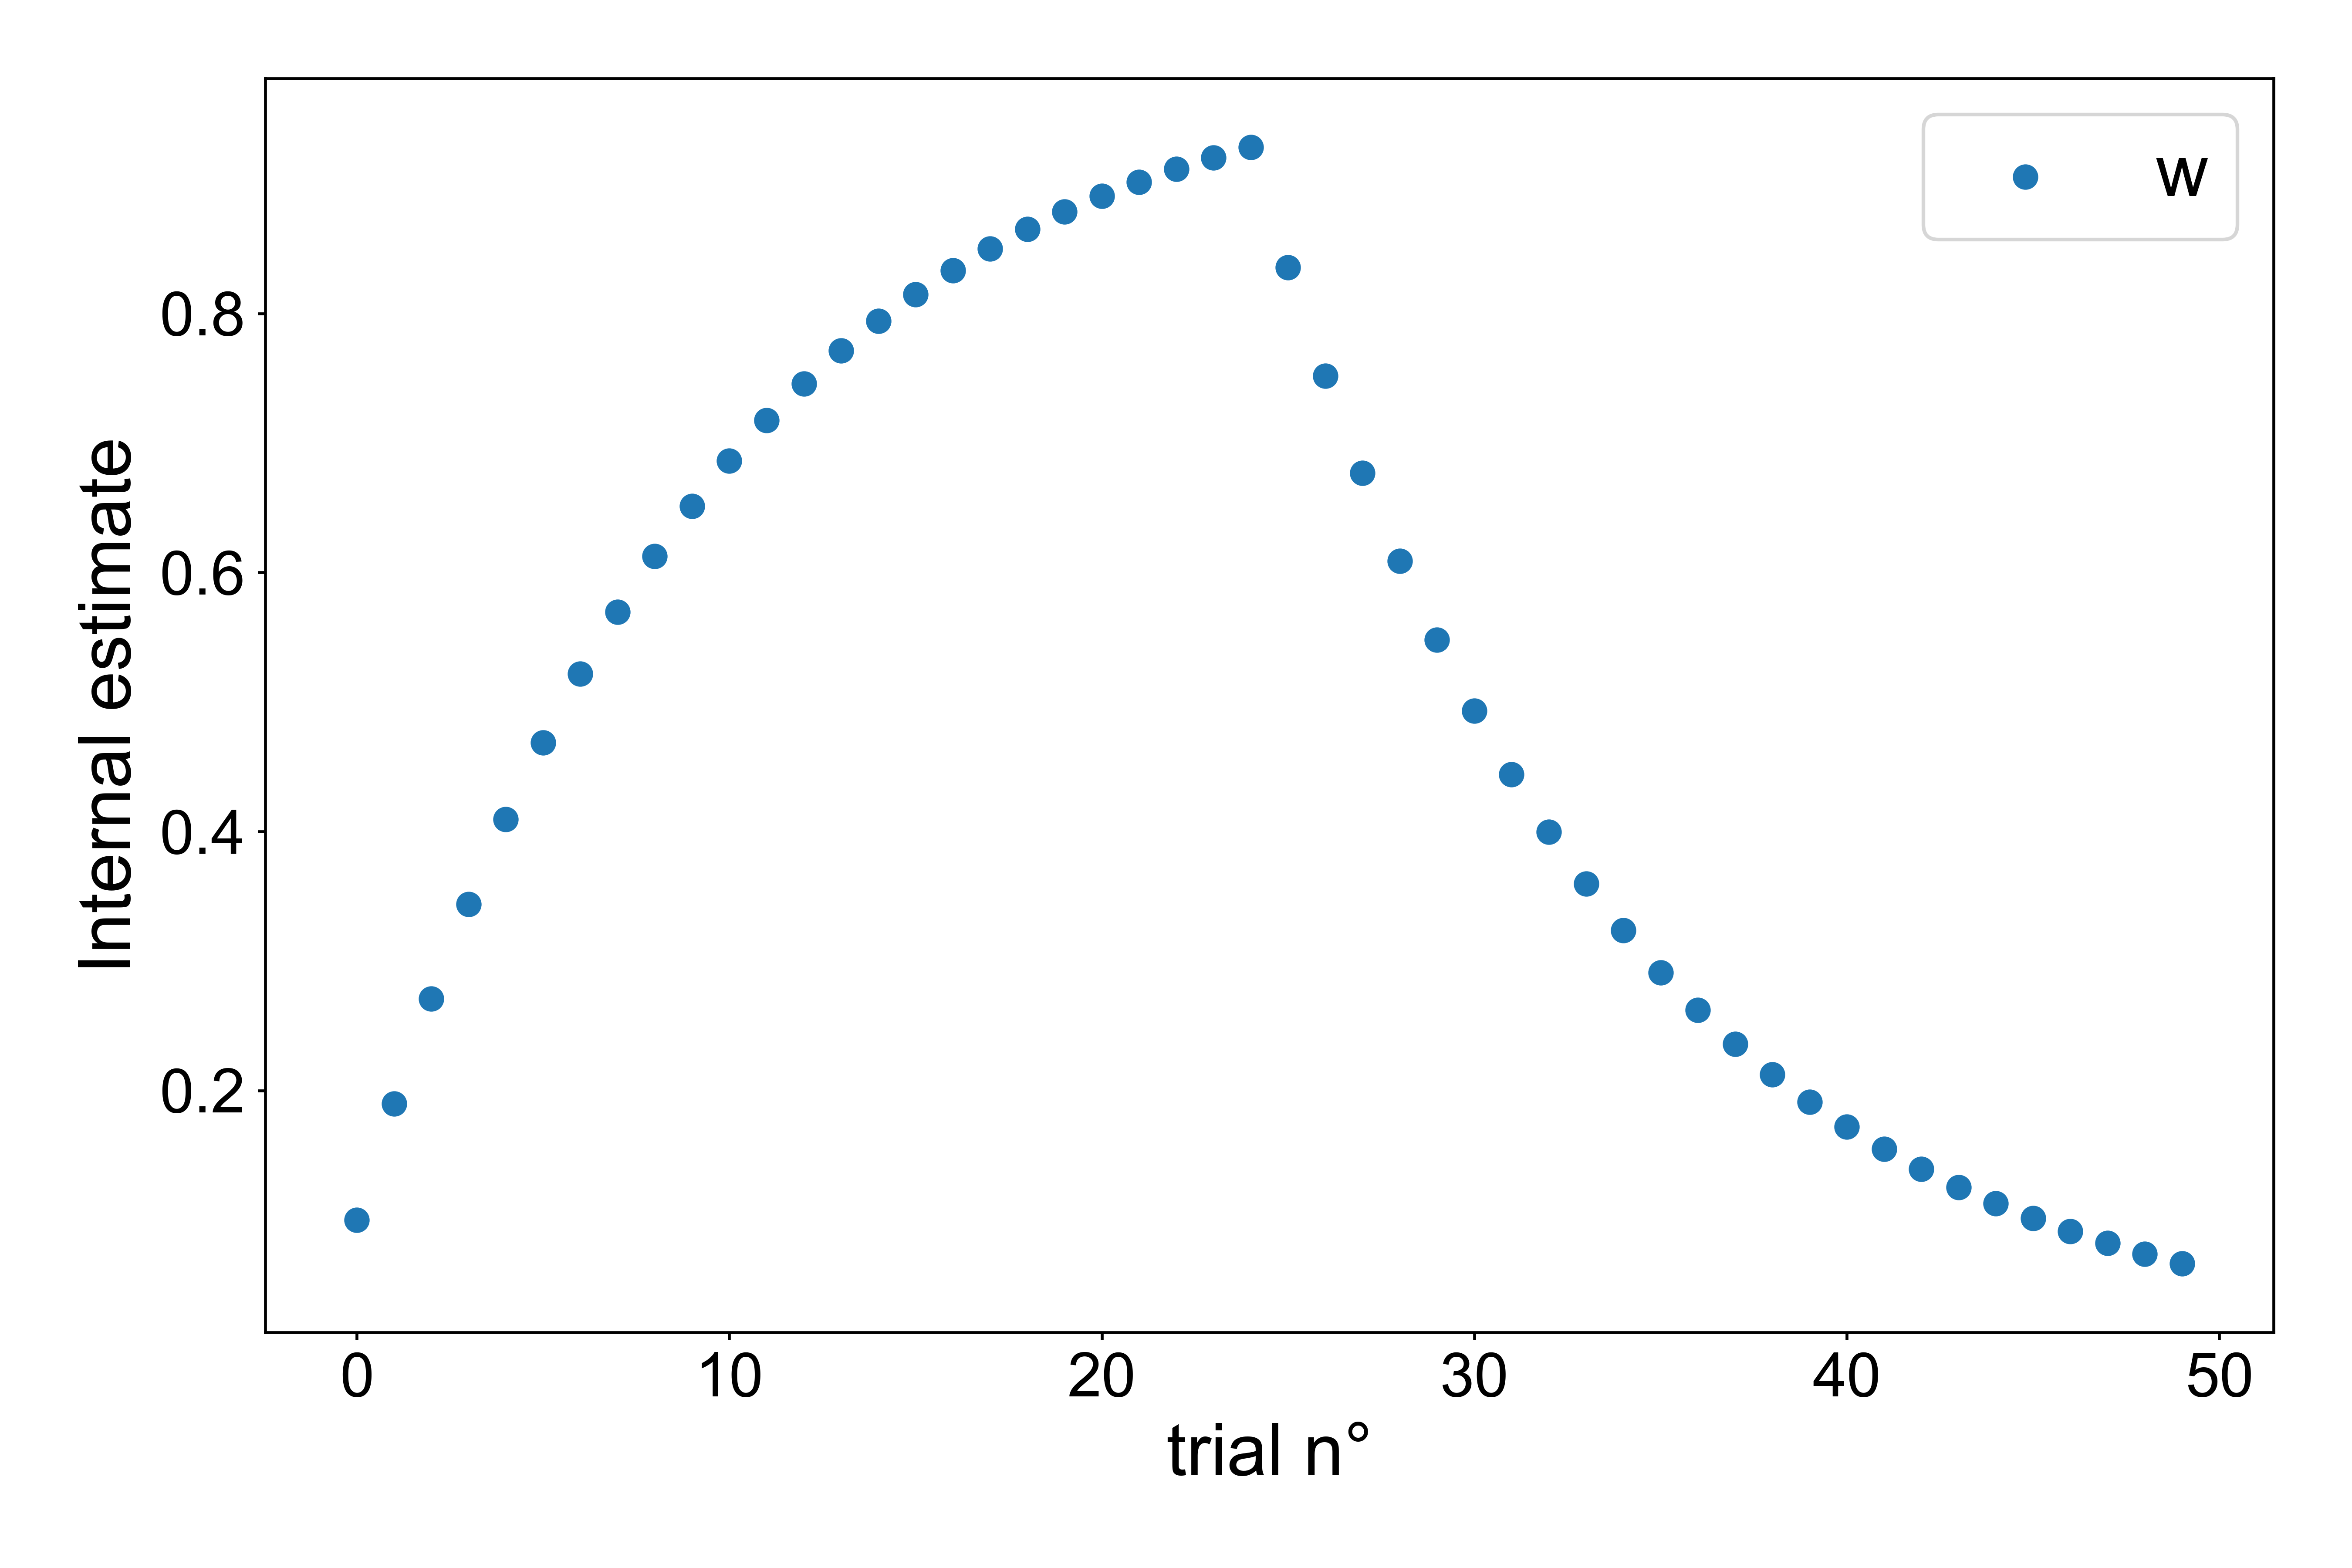
\includegraphics[width=.8\linewidth]{fig2_report2.png}
\caption[growing population]{Internal estimate $w$ updated with the delta-rule, as a function of the presence or absence of reward contingent with the US, with a learning rate $\epsilon = .1$.}\label{fig:fig1}
\end{figure}

In Figure \ref{fig:fig1}, the learning rate is fixed at .1, but the learning rate parameter modulates the speed at which the agent learn, \textit{i.e.} the weight of the current prediction error $\delta$ in updating. Figure \ref{fig:fig2} shows that a higher learning rate yields faster learning and faster extinction, which can be adaptive in a highly changing environment.

\begin{figure}[H]
\centering
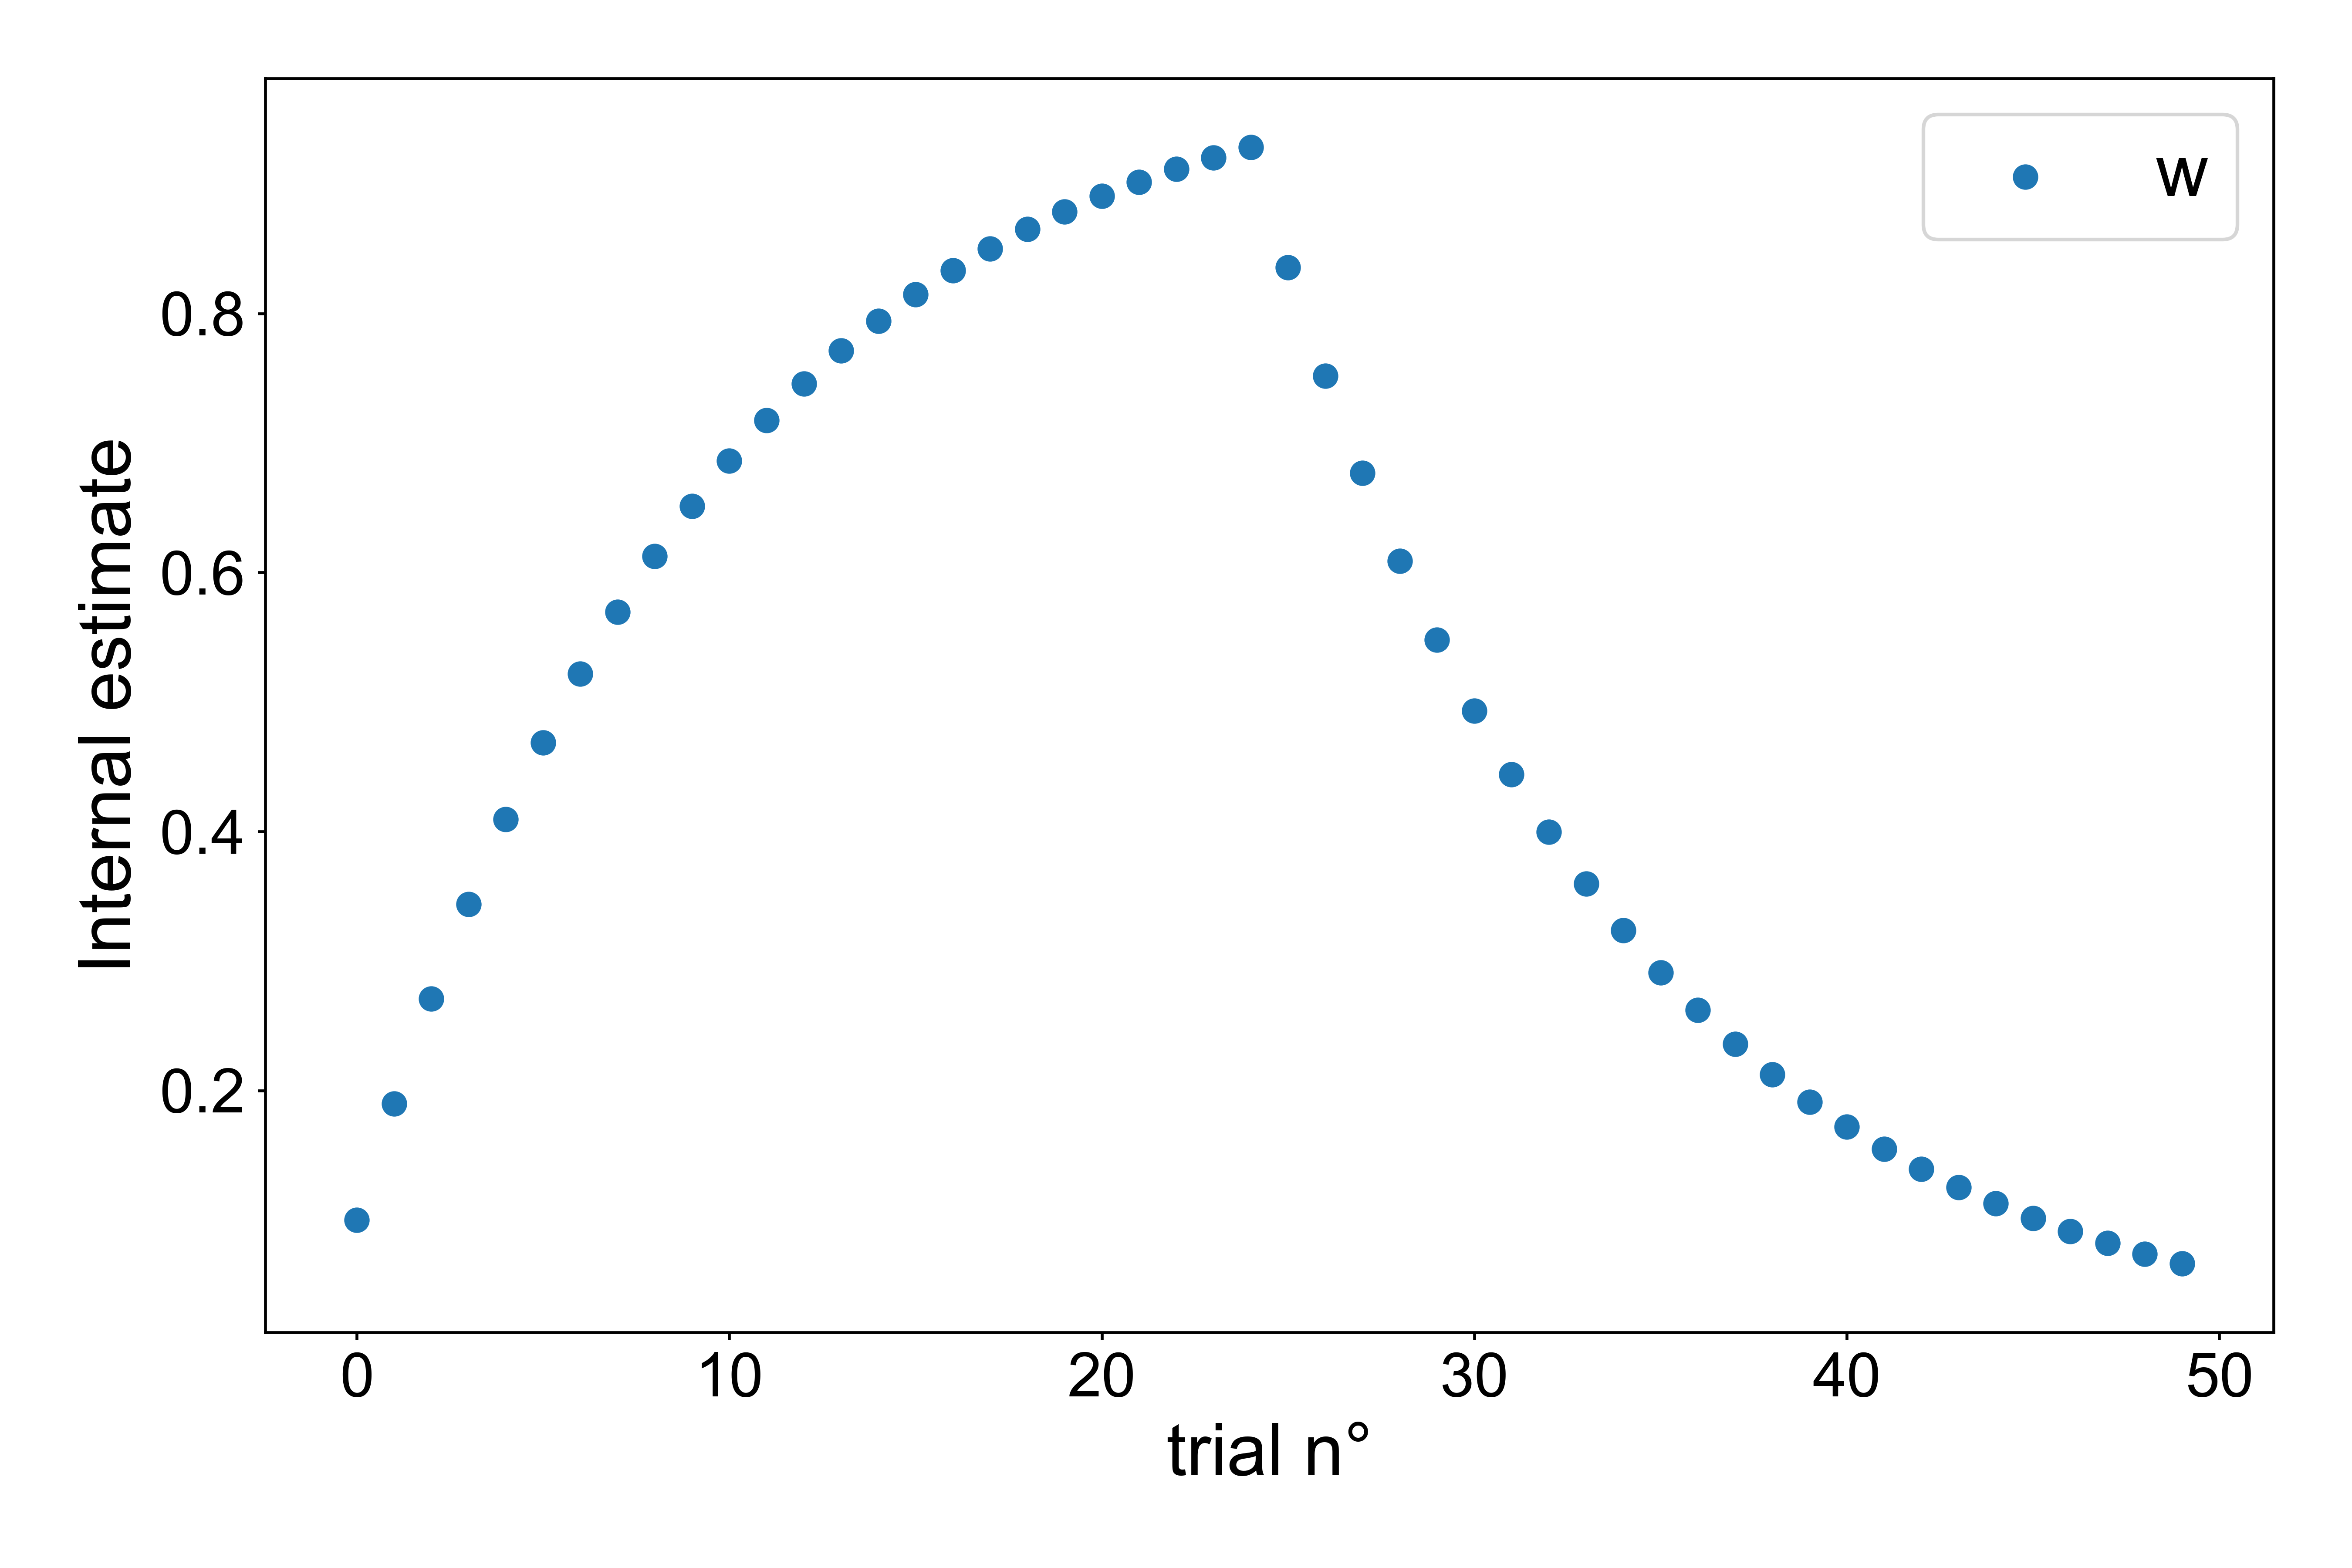
\includegraphics[width=.8\linewidth]{fig2_report3.png}
\caption[growing population]{Internal estimate $w$ updated with the delta-rule, as a function of the presence or absence of reward contingent with the US, with several different learning rates.}\label{fig:fig2}
\end{figure}

One might wonder if this simple model can still acount for learning in more complex environment with less certain contingencies. For instance, let's imagine a case where a reward has 50\% chance of appearing (Figure \ref{fig:fig3}). The internal estimate then represent in the same time the possible reward, and the probability of this possible reward, \textit{i.e.} the \textit{expected value} ($reward \times probability$) in economics terms. We see that the internal estimates fluctuates around .5, as it increases when the reward is present, and decreases when it is not. This rule can be somewhat efficient to learn in such an evironment, and/or compare several options, but it doesn't allow to ``represent" the environment as precisely, doesn't really match with behavioral results.

\begin{figure}[H]
\centering
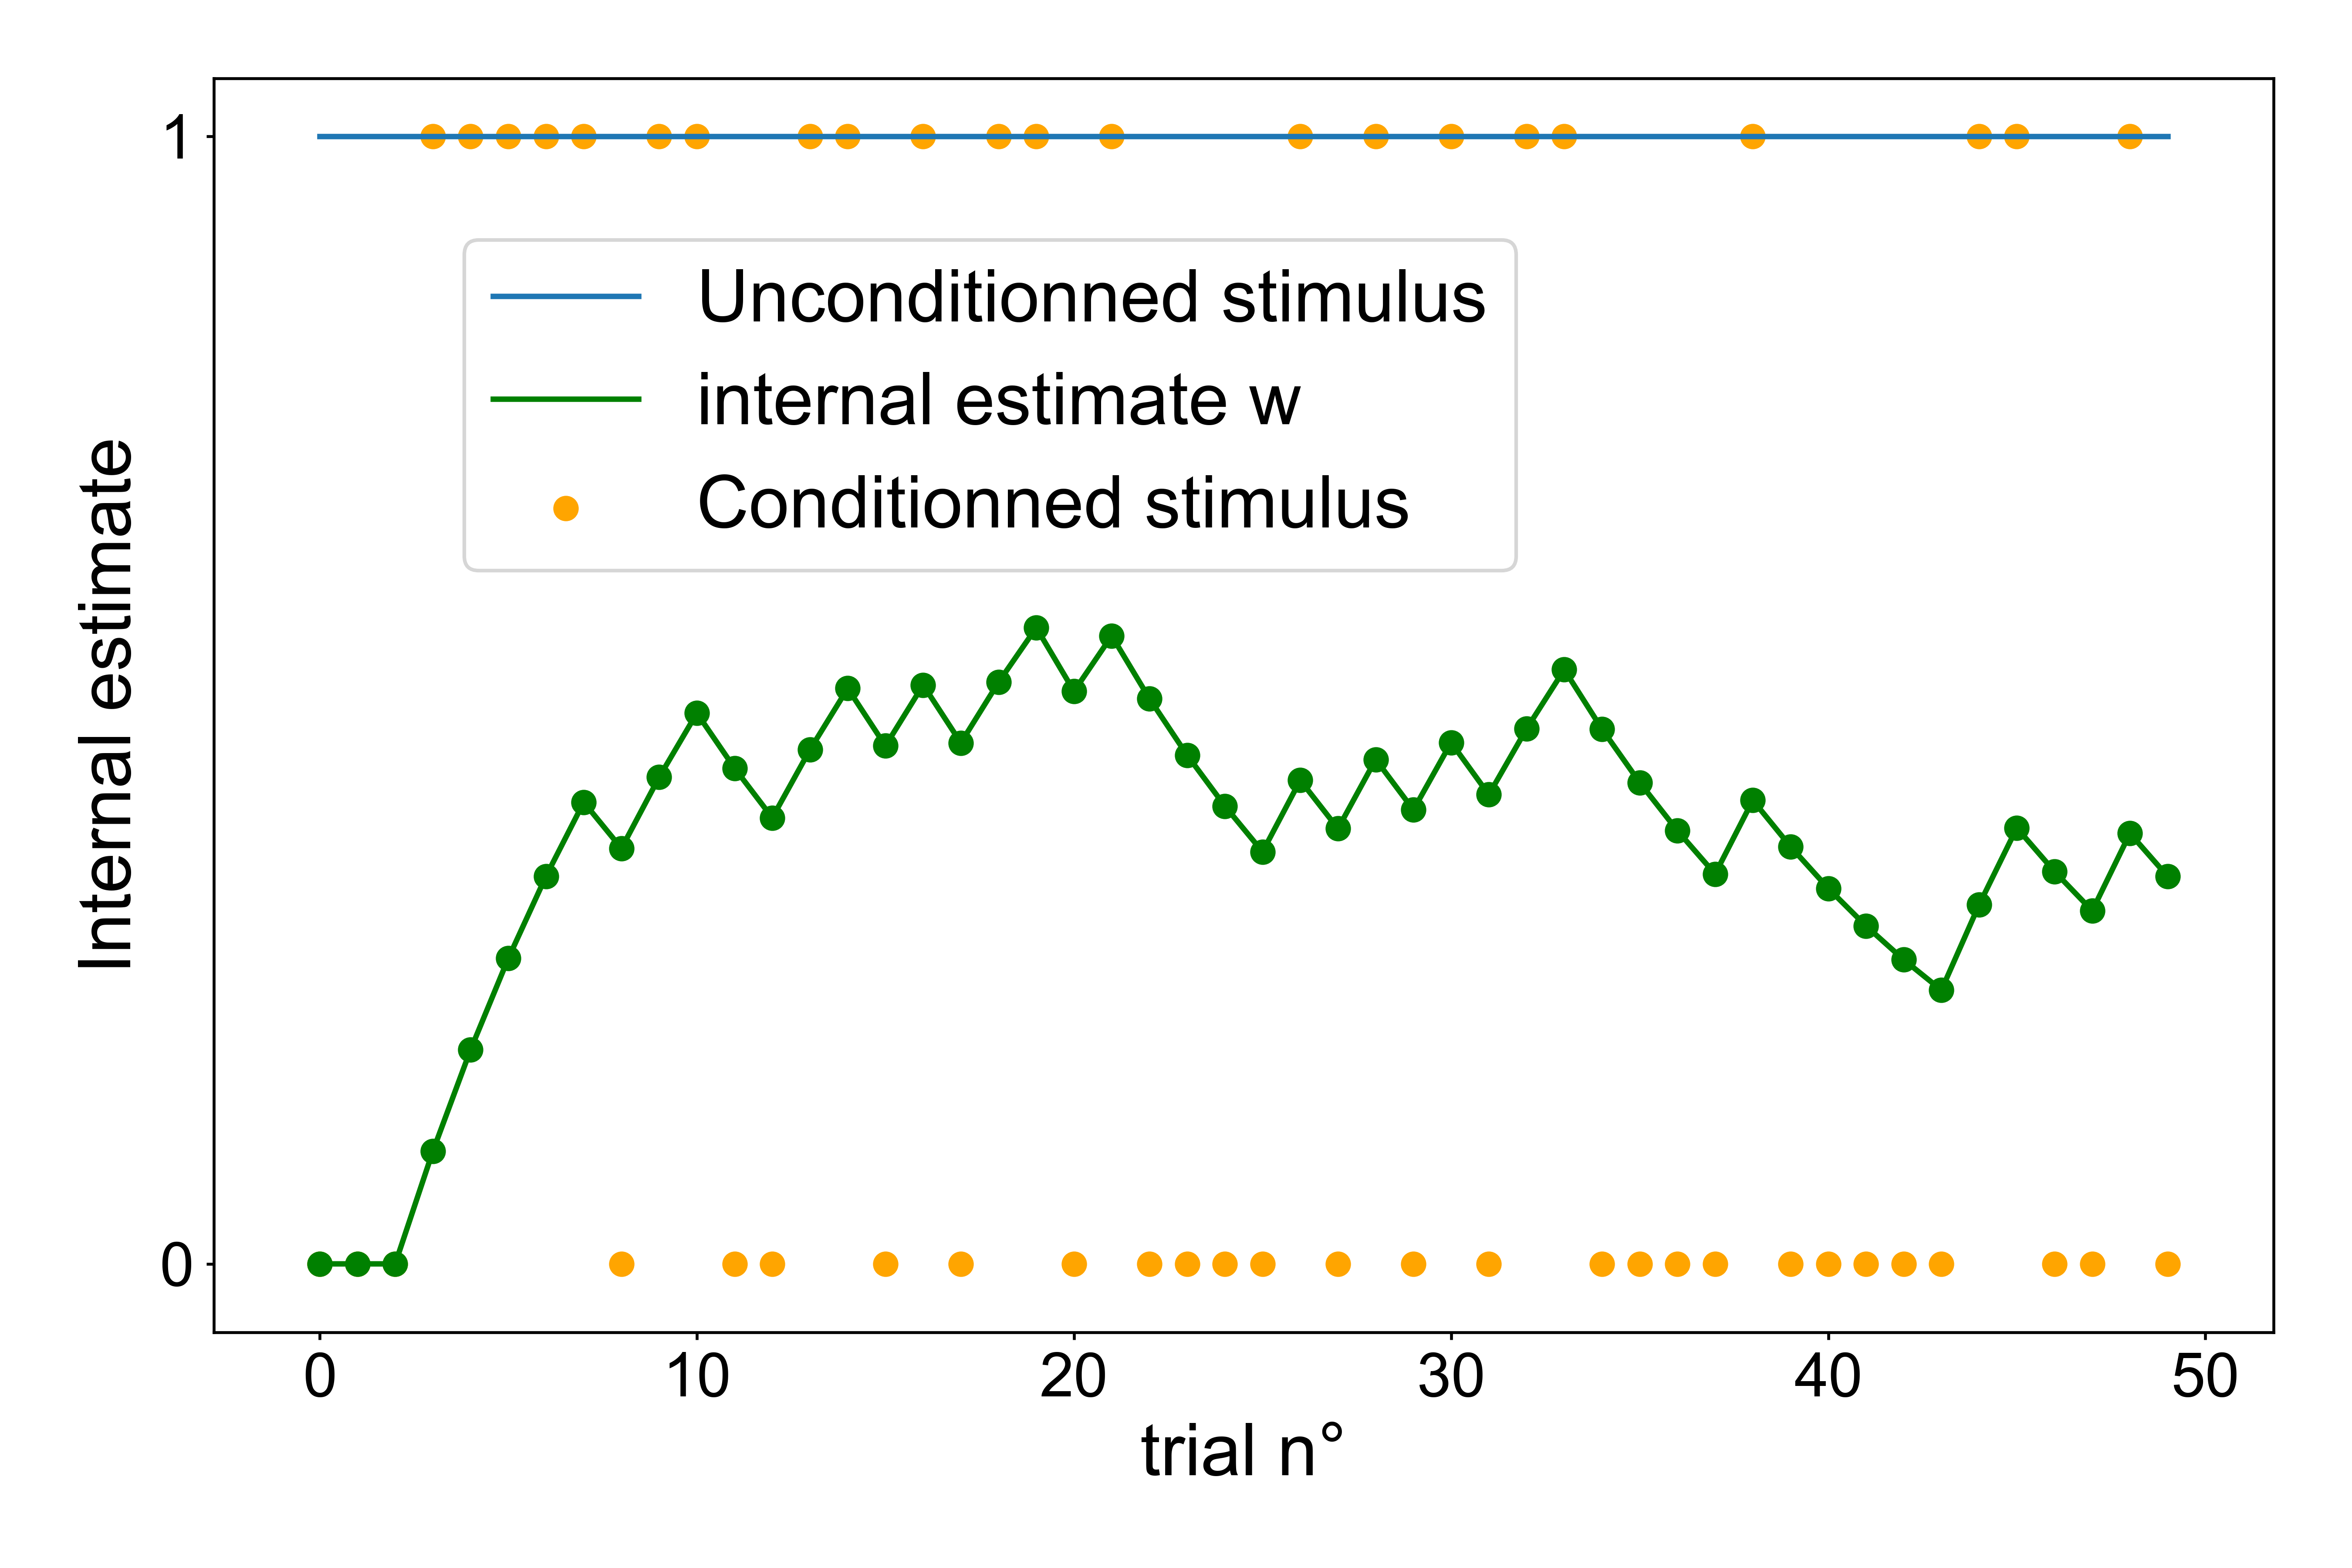
\includegraphics[width=.8\linewidth]{fig2_report5.png}
\caption[growing population]{Internal estimate $w$ in an uncertain environment, with $\epsilon = .1$.}\label{fig:fig3}
\end{figure}

Moreover, the model also explains easily some less obvious behavior like \textit{blocking}. If an agent has already learned an association between a US and a reward (\textit{i.e.} if the prediction error $\delta \rightarrow 0$), introducing a second US also contingent with the reward and the first US will not makje much difference. Indeed, the reward is already explained by the first US, and the prediction error $\delta$ is so low that the second internal estimate $w_2$ will barely be updated (Figure \ref{fig:fig4}).

\begin{figure}[H]
\centering
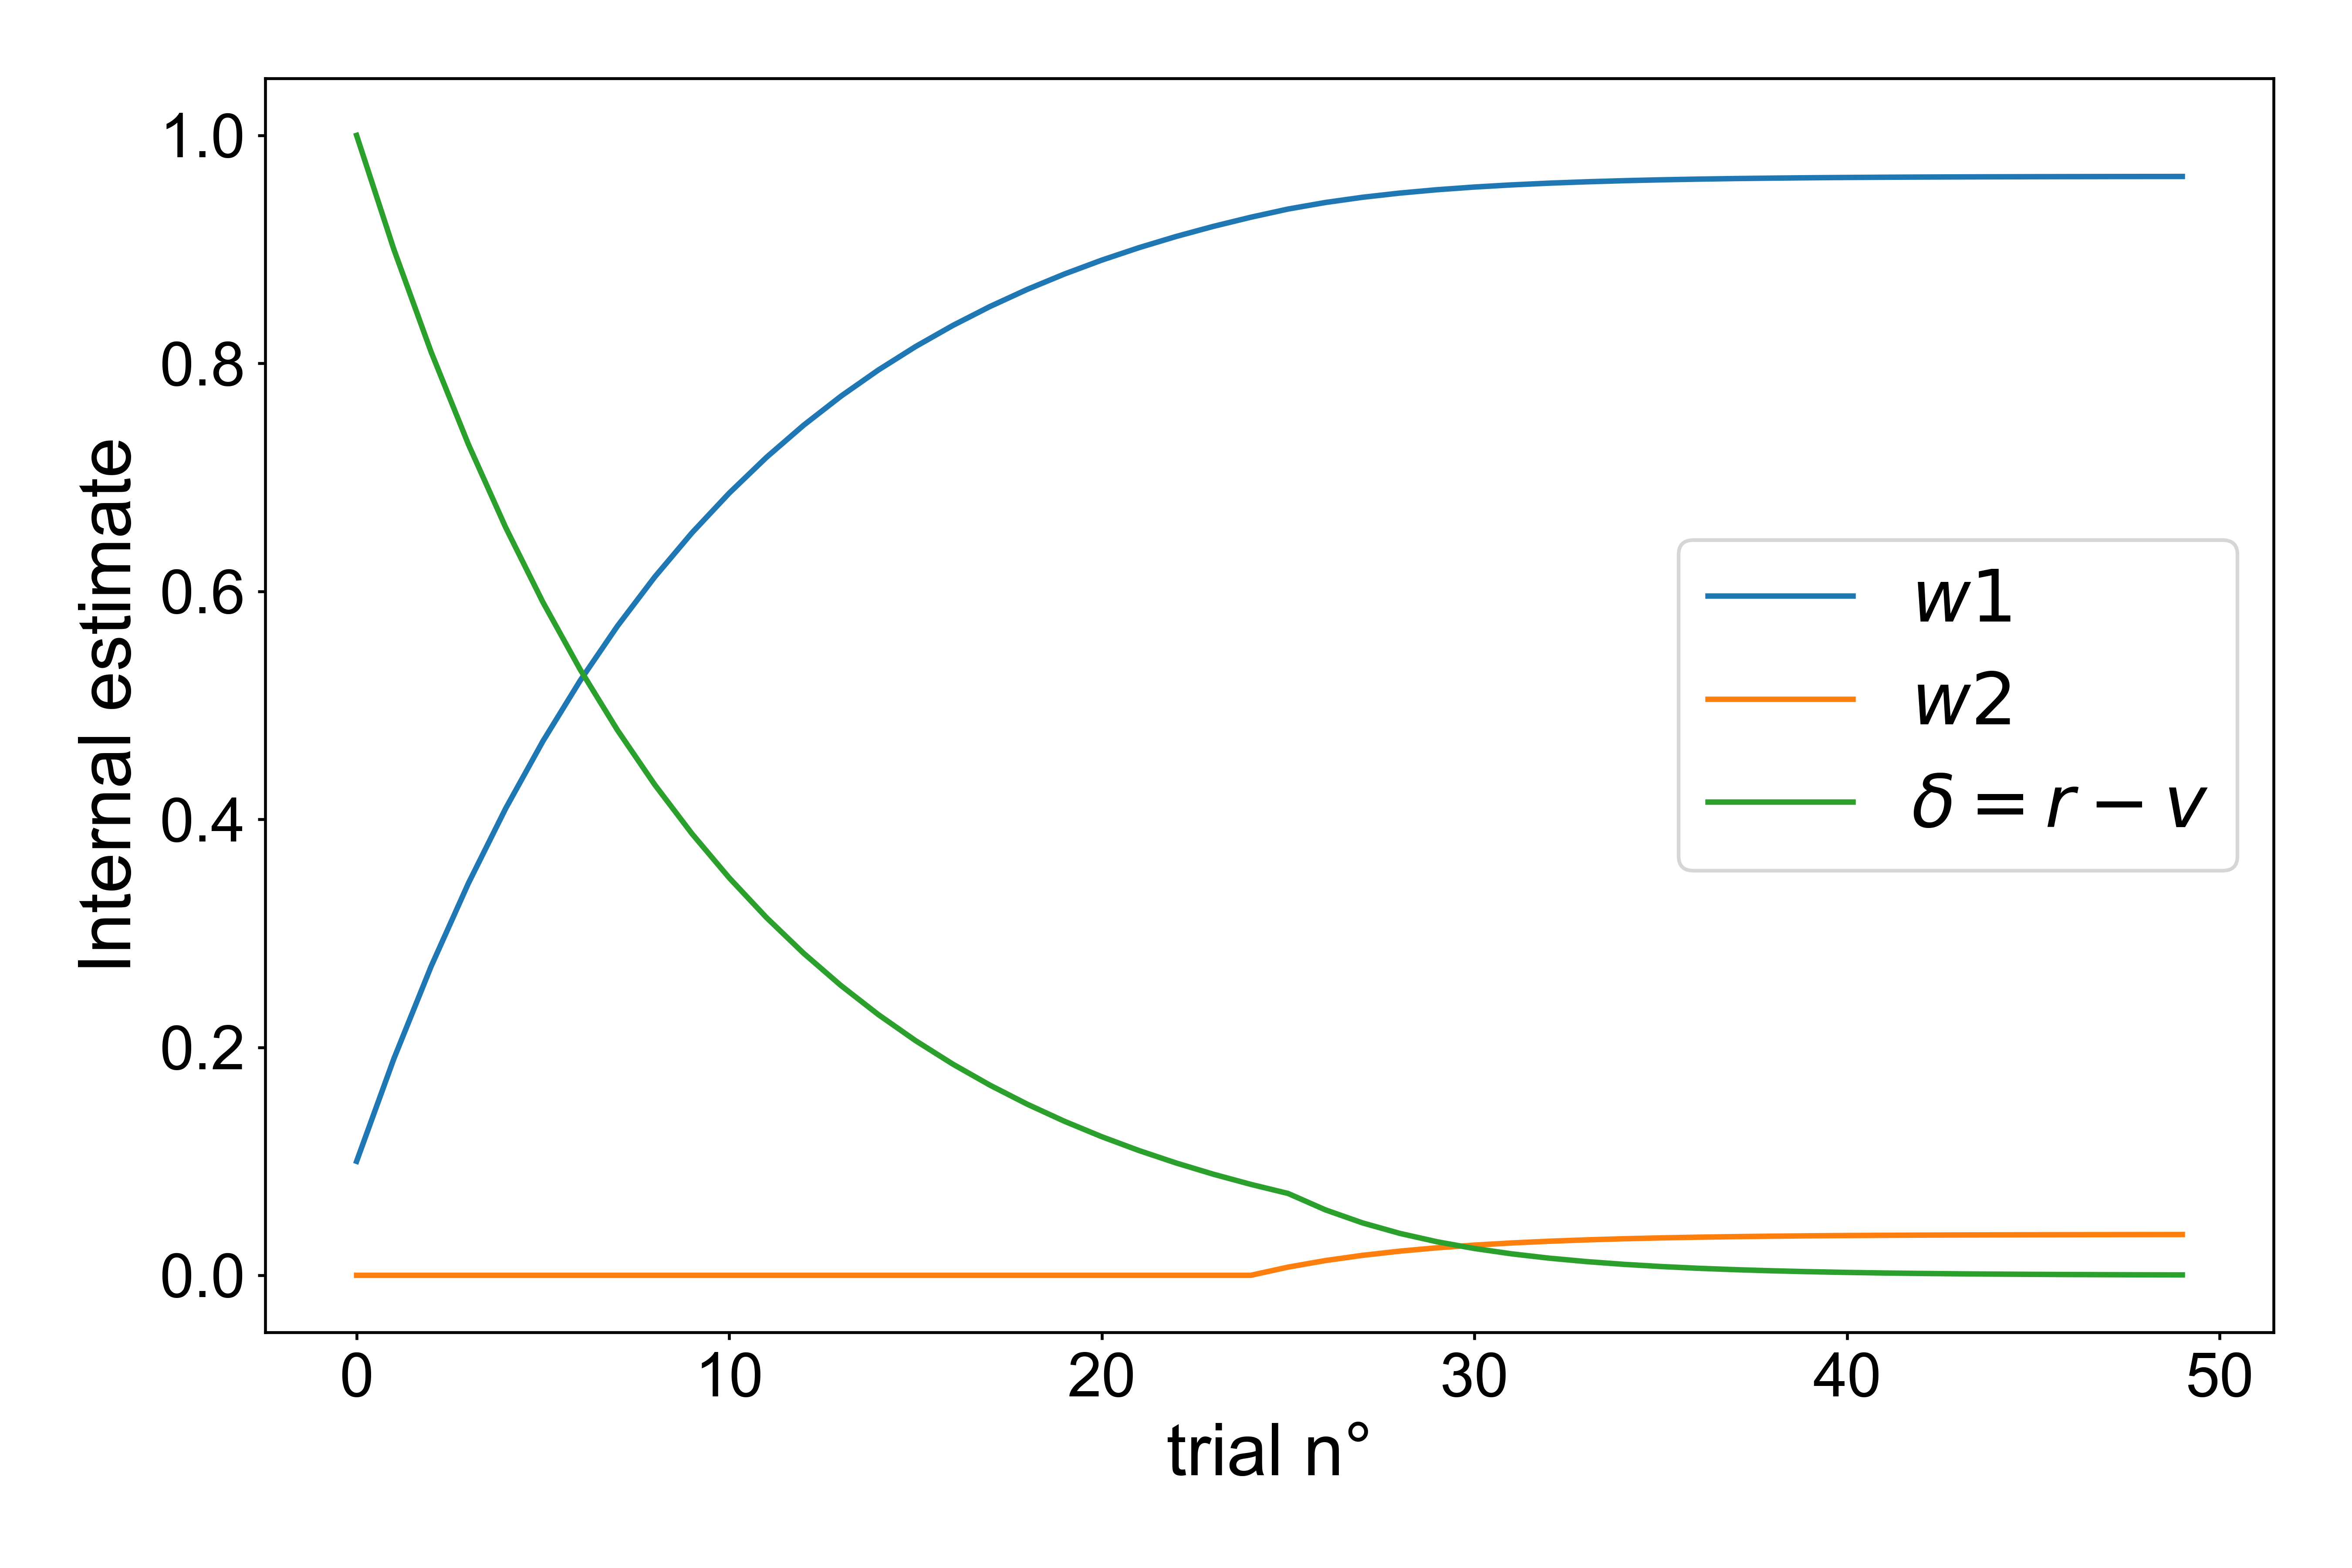
\includegraphics[width=.8\linewidth]{fig2_report6.png}
\caption[growing population]{Internal estimates and prediction error, with a second US introduced at trial 25. $\epsilon = .1$.}\label{fig:fig4}
\end{figure}

Similarly, if we have two US with different learning rate, we will come upon an \textit{undershadowing} phenomenon. The US with the highest learning rate will update more rapidly, and end up explaining more of the reward, \textit{i.e.} having a higher internal estimate (Figure \ref{fig:fig5}). One can imagine such phenomena can be observed when the US used is not so ``unconditioned", and is somewhat hardwired. For instance, a picture of a banana tree might be more easily associated with a reward than a neutral picture, itself more easily associated with a reward than a picture of a spider.

\begin{figure}[H]
\centering
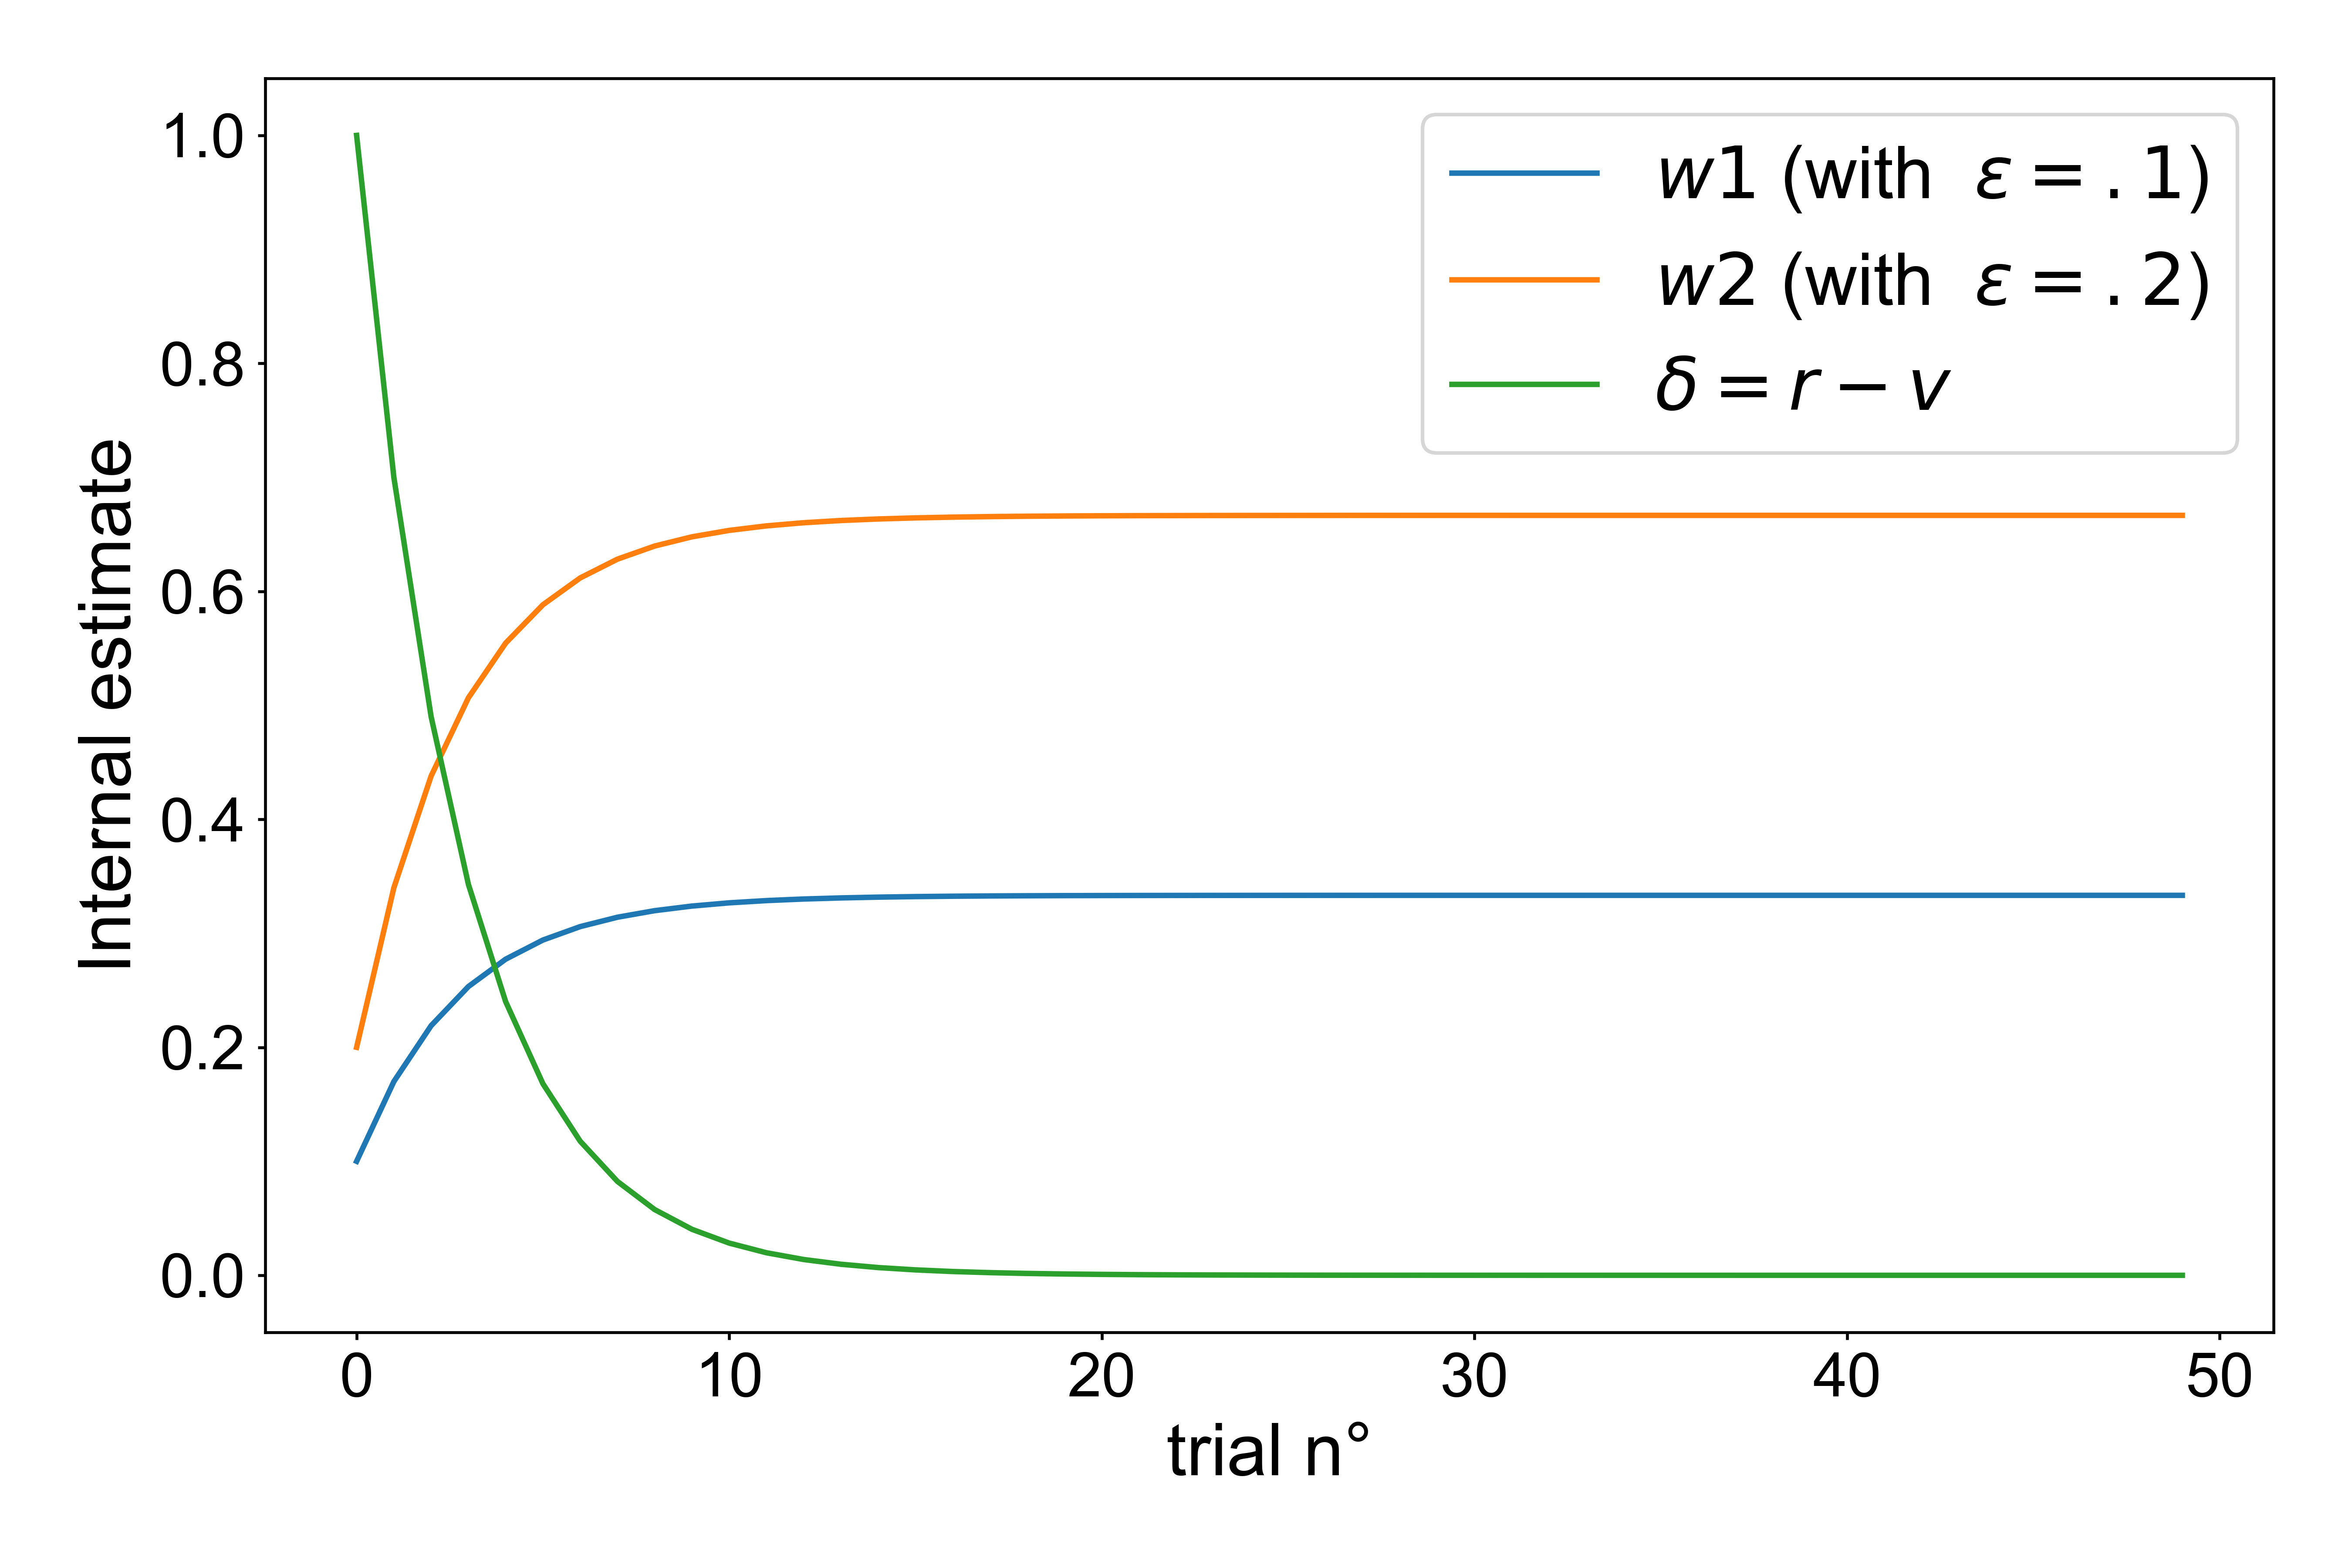
\includegraphics[width=.8\linewidth]{fig2_report7.png}
\caption[growing population]{Internal estimates and prediction error of two US with different learning rates.}\label{fig:fig5}
\end{figure}


However, some phenomena like \textit{secondary conditioning} can not be explained by the Rescorla-Wagner rule.
 %----------------------------------------------------------------------------------------
 %	SECTION 2
 %----------------------------------------------------------------------------------------
 \section{Decision Making}
\indent\indent In addition to learning, a lot of focus has been on modeling decision making. One reason is that human behavior is ``irrational", in the sense that we don't always optimize our returns, in a way that seems counter-adaptive. Many evolutionary theorists and (neuro-)behavioral economists have tried to tackle the problem. However, one can ``fit" behavioral data with some very simple computational models.\\

 \subsection{Policy}

\indent\indent First, modeling probability of action seems more suited to a behavioral problem. For instance, the softmax (or Gibbs) policy, is a simple formula designed to compute the probability of an action given a field of possible actions, based on their respective internal estimates (Cf Section 2). Let's take the textbook example of a foraging bee, having the possibility of going to either blue or yellow flowers. Let $m_b$ and $m_y$ be the internal estimates of blue and yellow flowers respectively, $\beta$ the temperature parameter (explained later), and $p_b$ the probability of choosing a blue flower:

\begin{align*}
  p_b &=   \frac{1} {1 + e^{\beta (m_y - m_b)}} \\
      &= \frac{e^{\beta m_b}} {e^{\beta m_b} + e^{\beta m_y}}
\end{align*}

The $\beta$ parameter is also refered to as the ``exploitation-exploration trade-off" parameter. Figure \ref{fig:fig6} shows indeed that the higher is $\beta$, the lower is the probability to choose an option which doesn't yield the highest return, \textit{i.e.} to ``explore". On the contrary, the closer $\beta$ is to zero, the higher the tendency of the agent to explore inferior options, \textit{i.e.} to choose regardless of the internal estimate difference. Figure \ref{fig:fig7} shows that different $\beta$ for a same difference changes the probability of choosing a blue flower, with a negative $\beta$ yielding a tendency to choose the flower with the lowest return.
\\
 The explore-exploit distinction is paradigmatic in decision science, and the $\beta$ parameter changes depending on the agent, but also on the context (similarly to the learning rate $\epsilon$ in Section 2).

\begin{figure}[H]
\centering
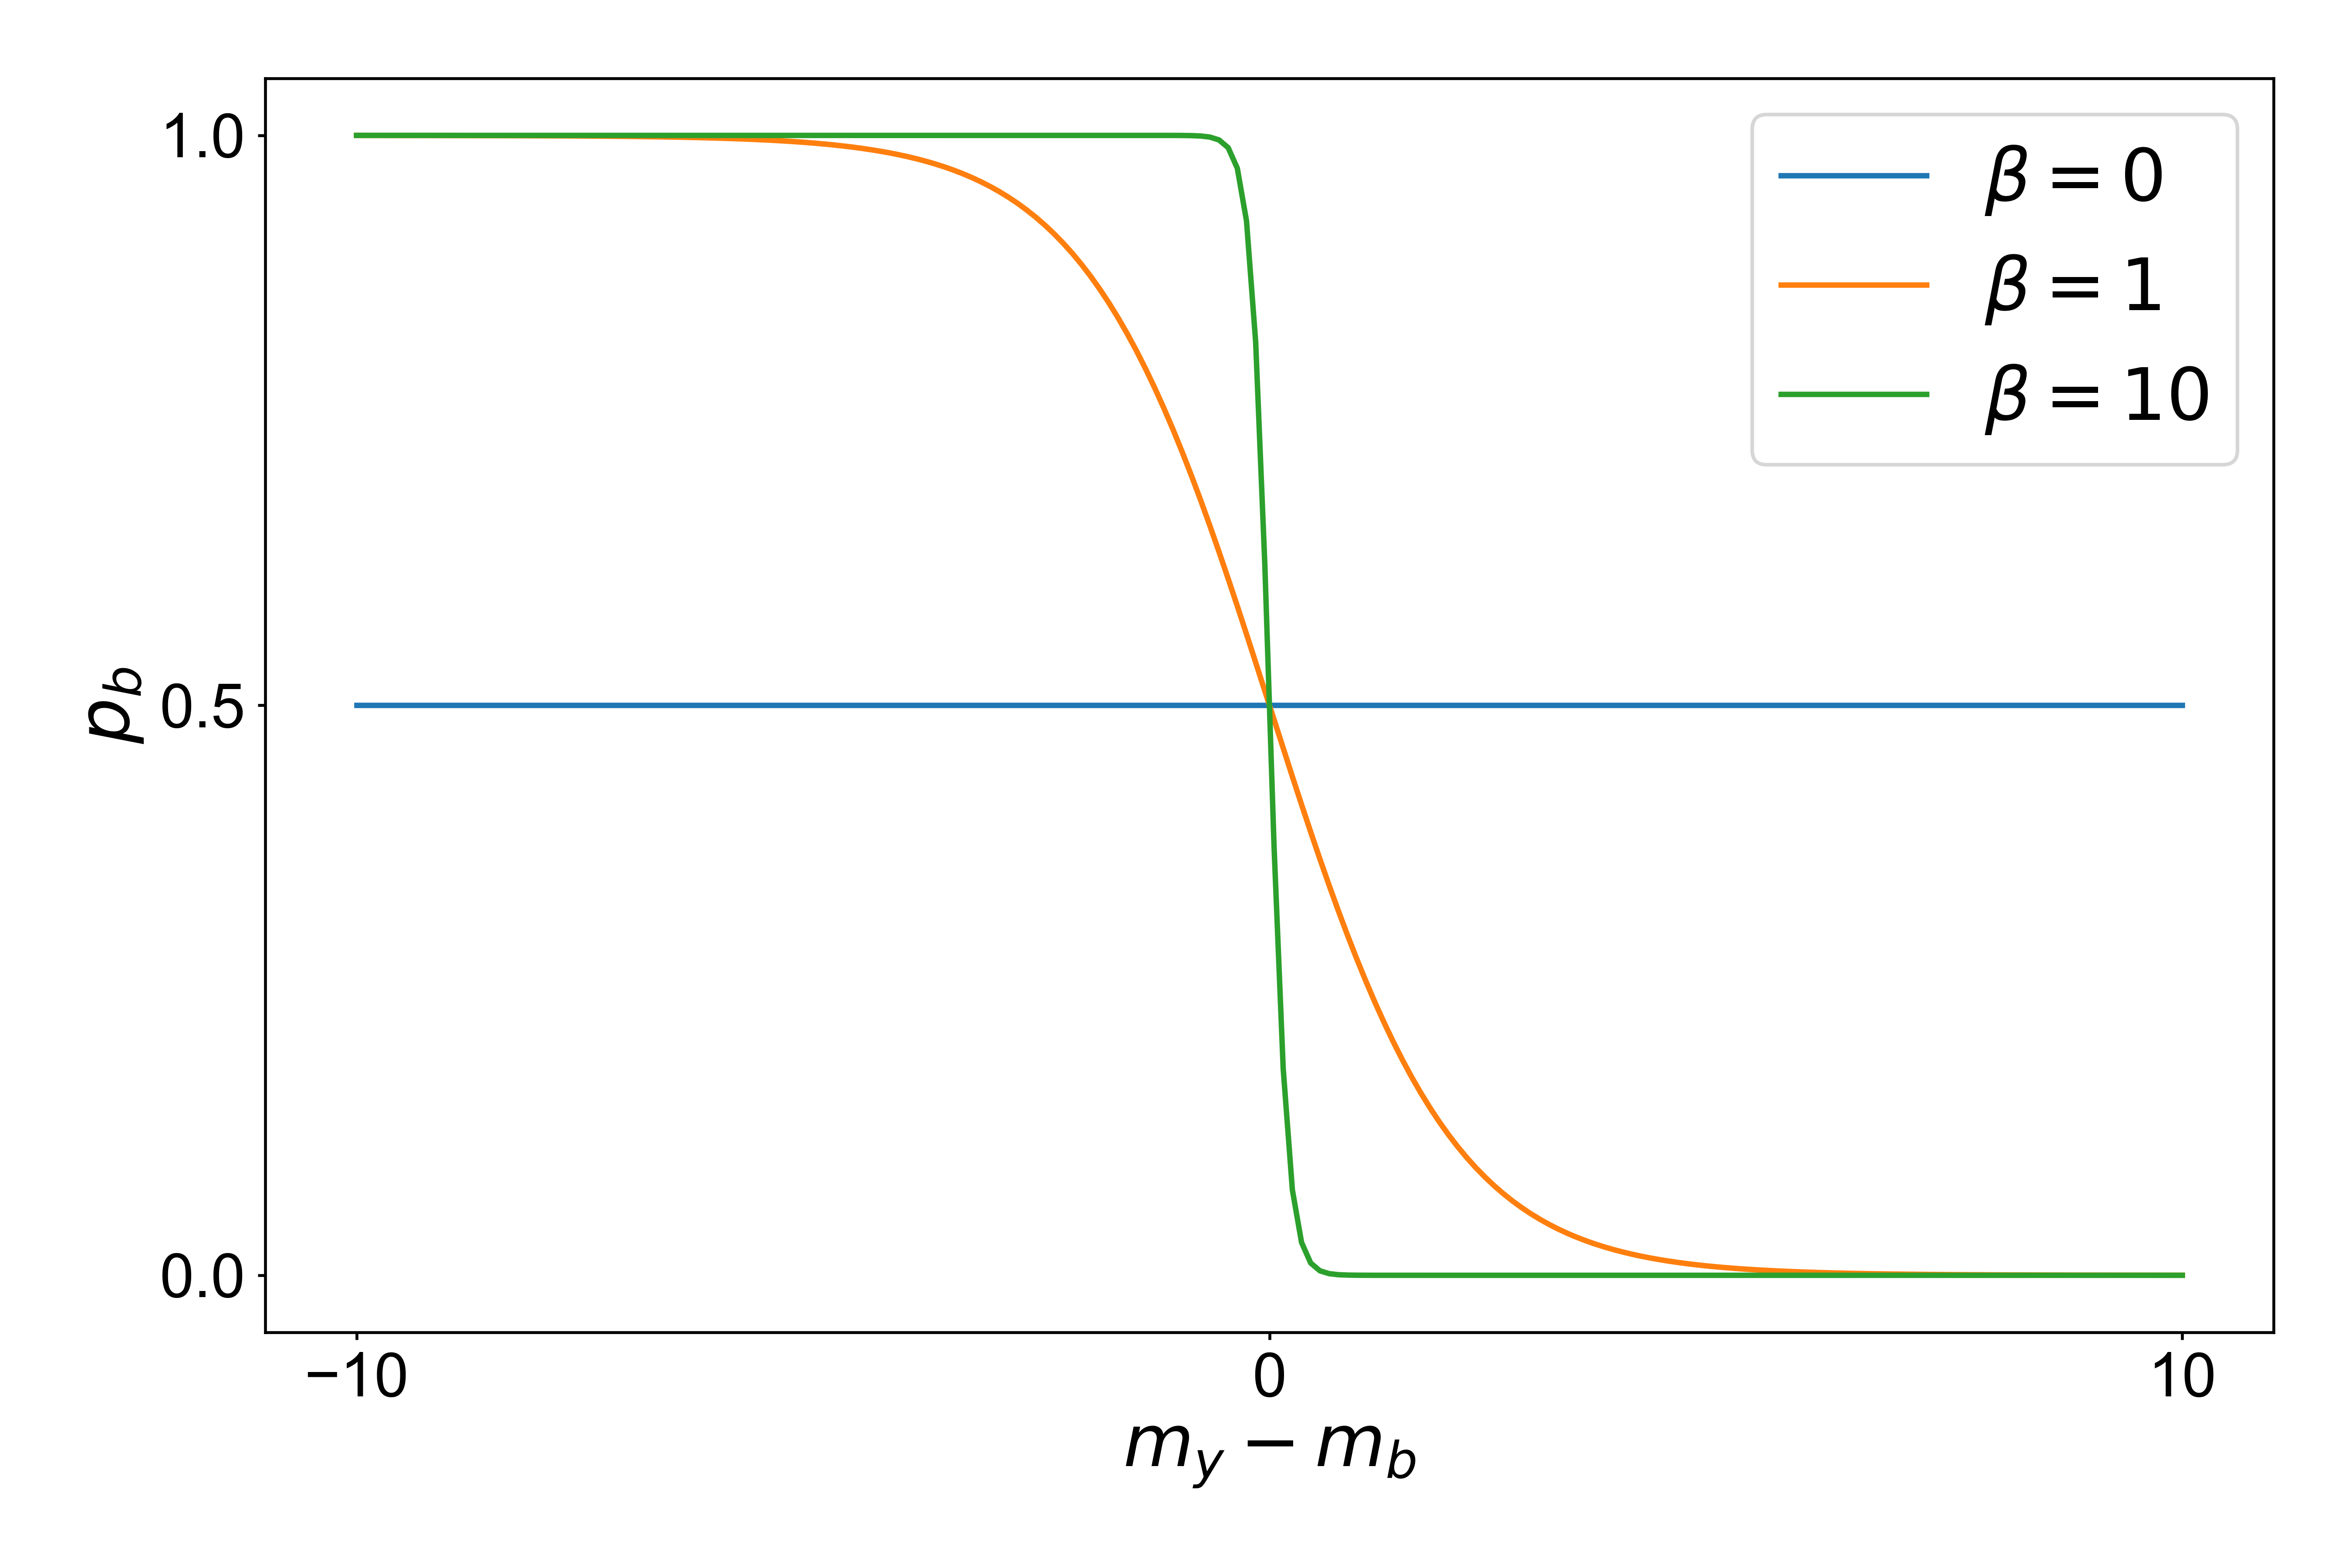
\includegraphics[width=.8\linewidth]{fig2_report9.png}
\caption[growing population]{Probability of choosing a blue flower, depending on the difference between the internal estimates of blue and yellow flowers, and on the $\beta$ parameter.}\label{fig:fig6}
\end{figure}

\begin{figure}[H]
\centering
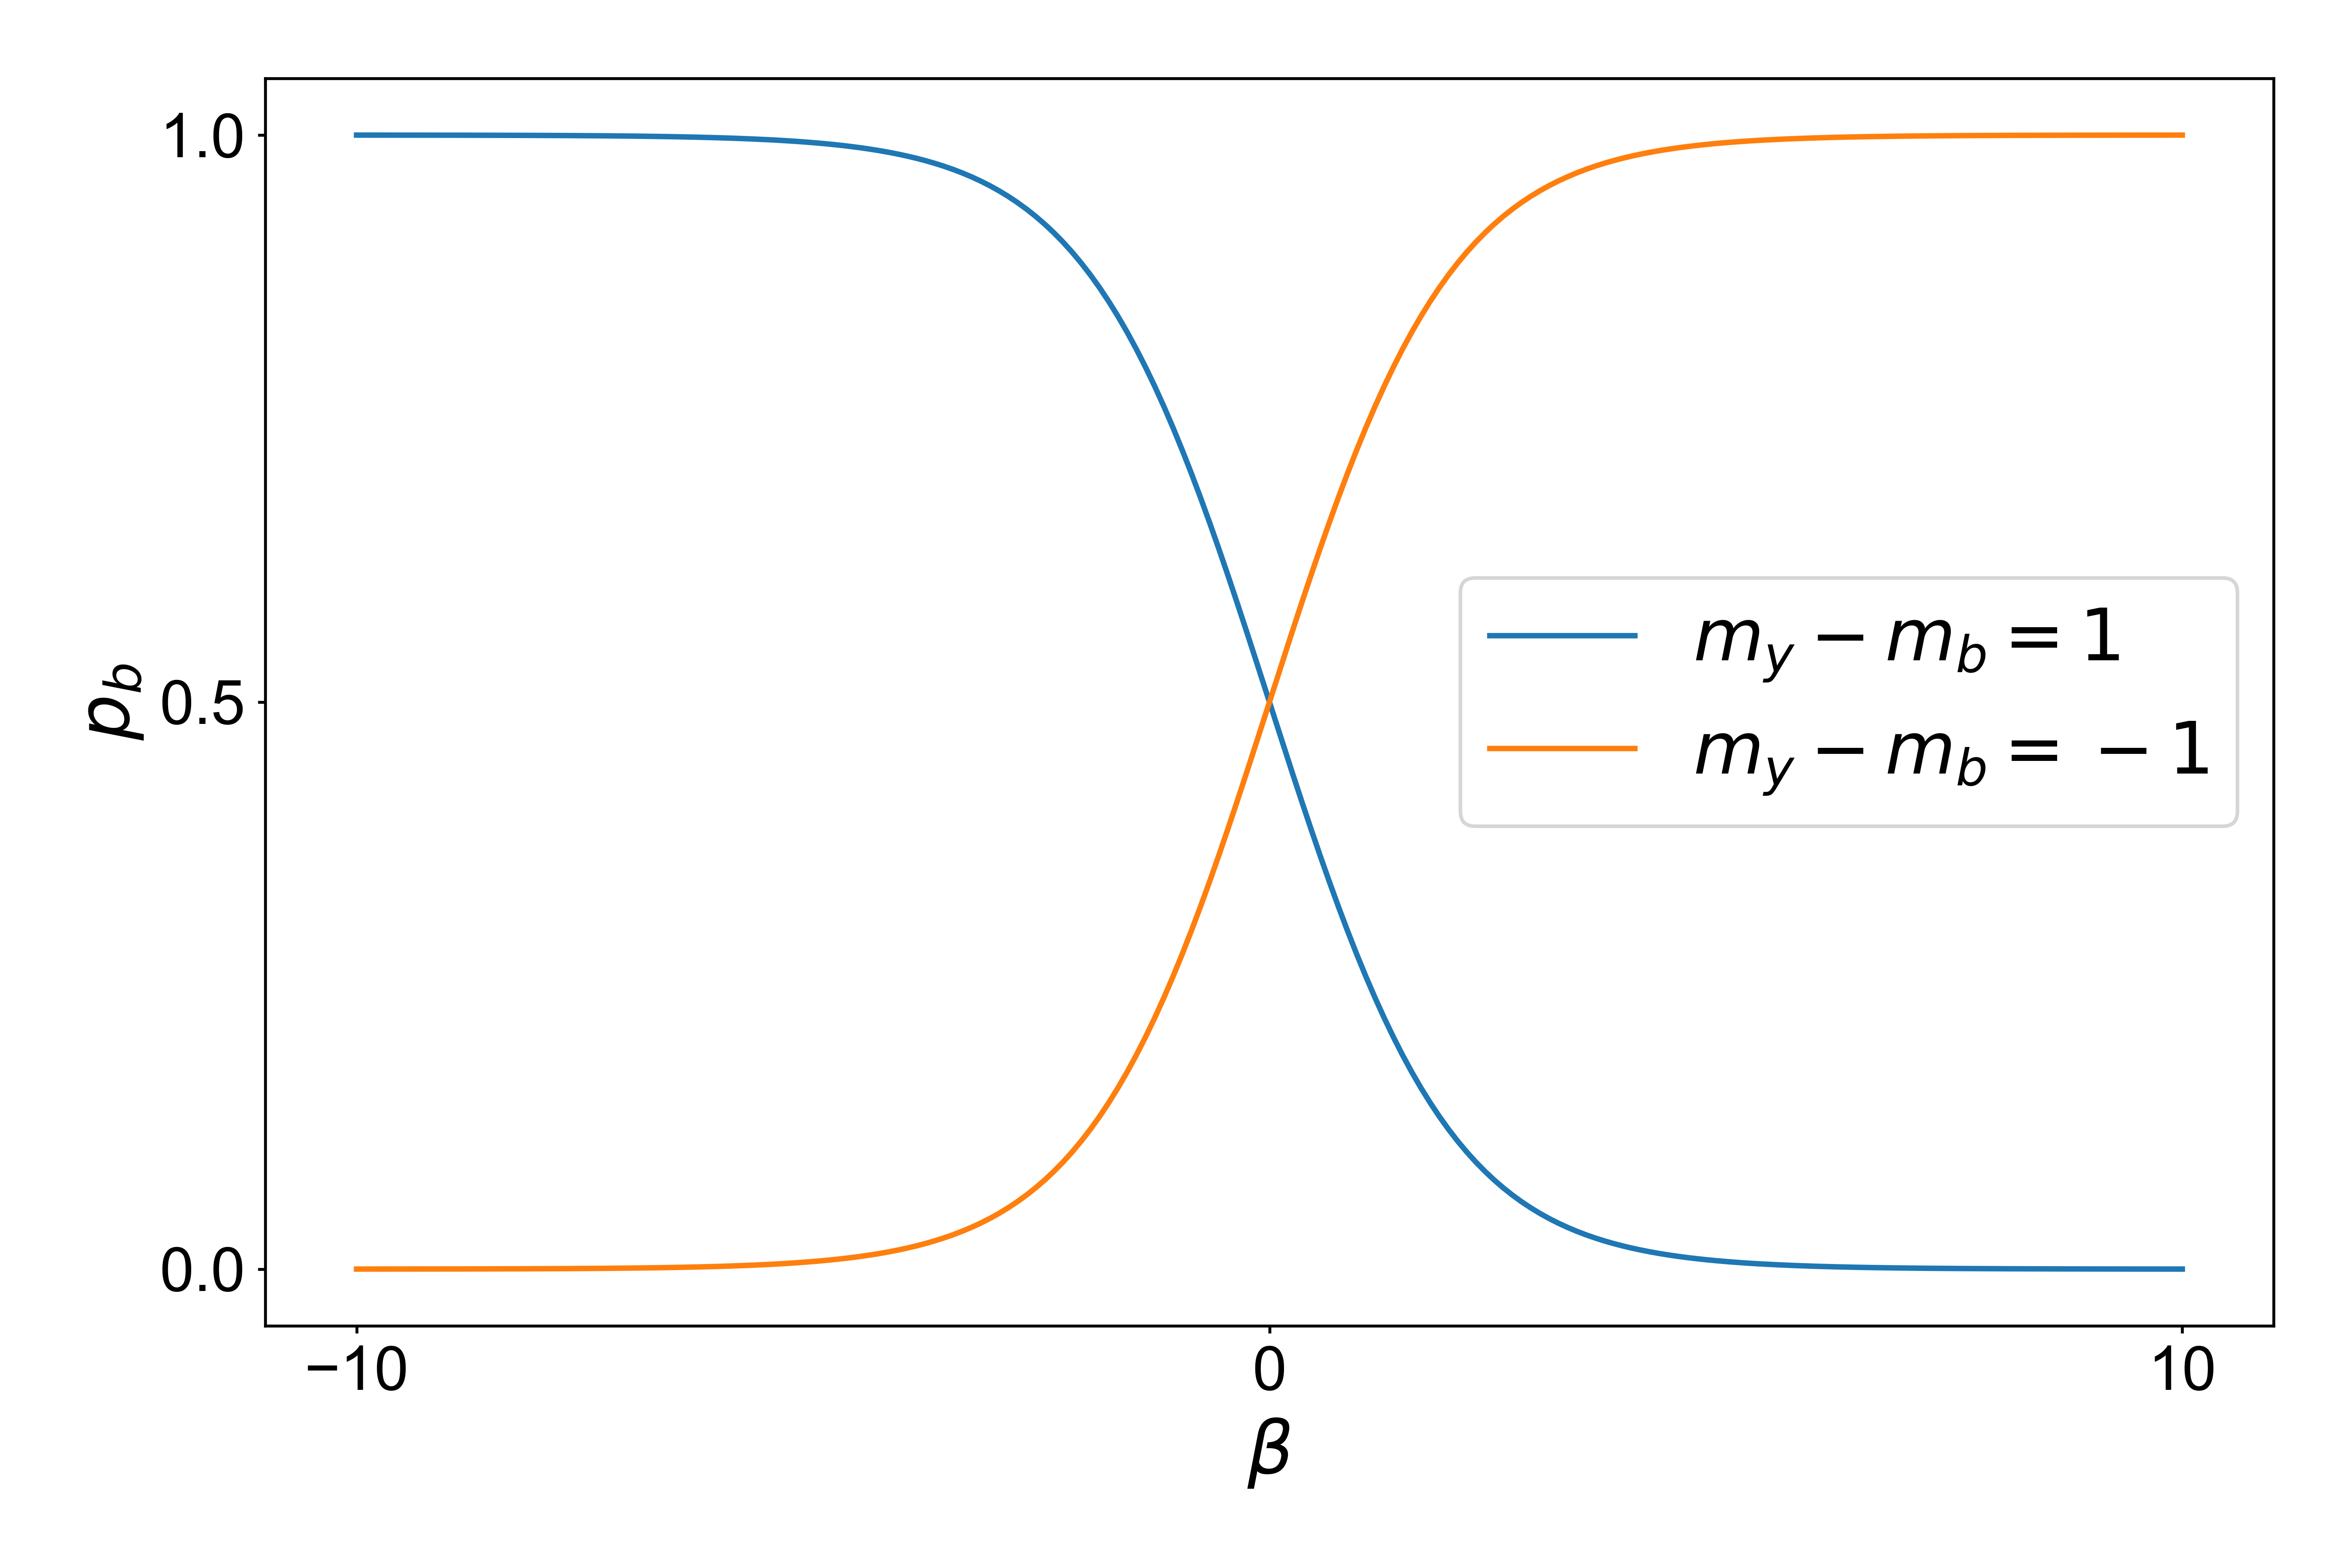
\includegraphics[width=.8\linewidth]{fig2_report10.png}
\caption[growing population]{Probability of choosing a blue flower, depending on the difference between the internal estimates of blue and yellow flowers, and on the $\beta$ parameter.}\label{fig:fig7}
\end{figure}

If we imagine that the bee as for fixed internal estimates $m_b = 0$ and $m_y = 5$, the choice pattern will be different for different $\beta$s: much less likely to choose the lower pay-off option with a higher $\beta$ (Figure \ref{fig:fig8}).

\begin{figure}[H]
\centering
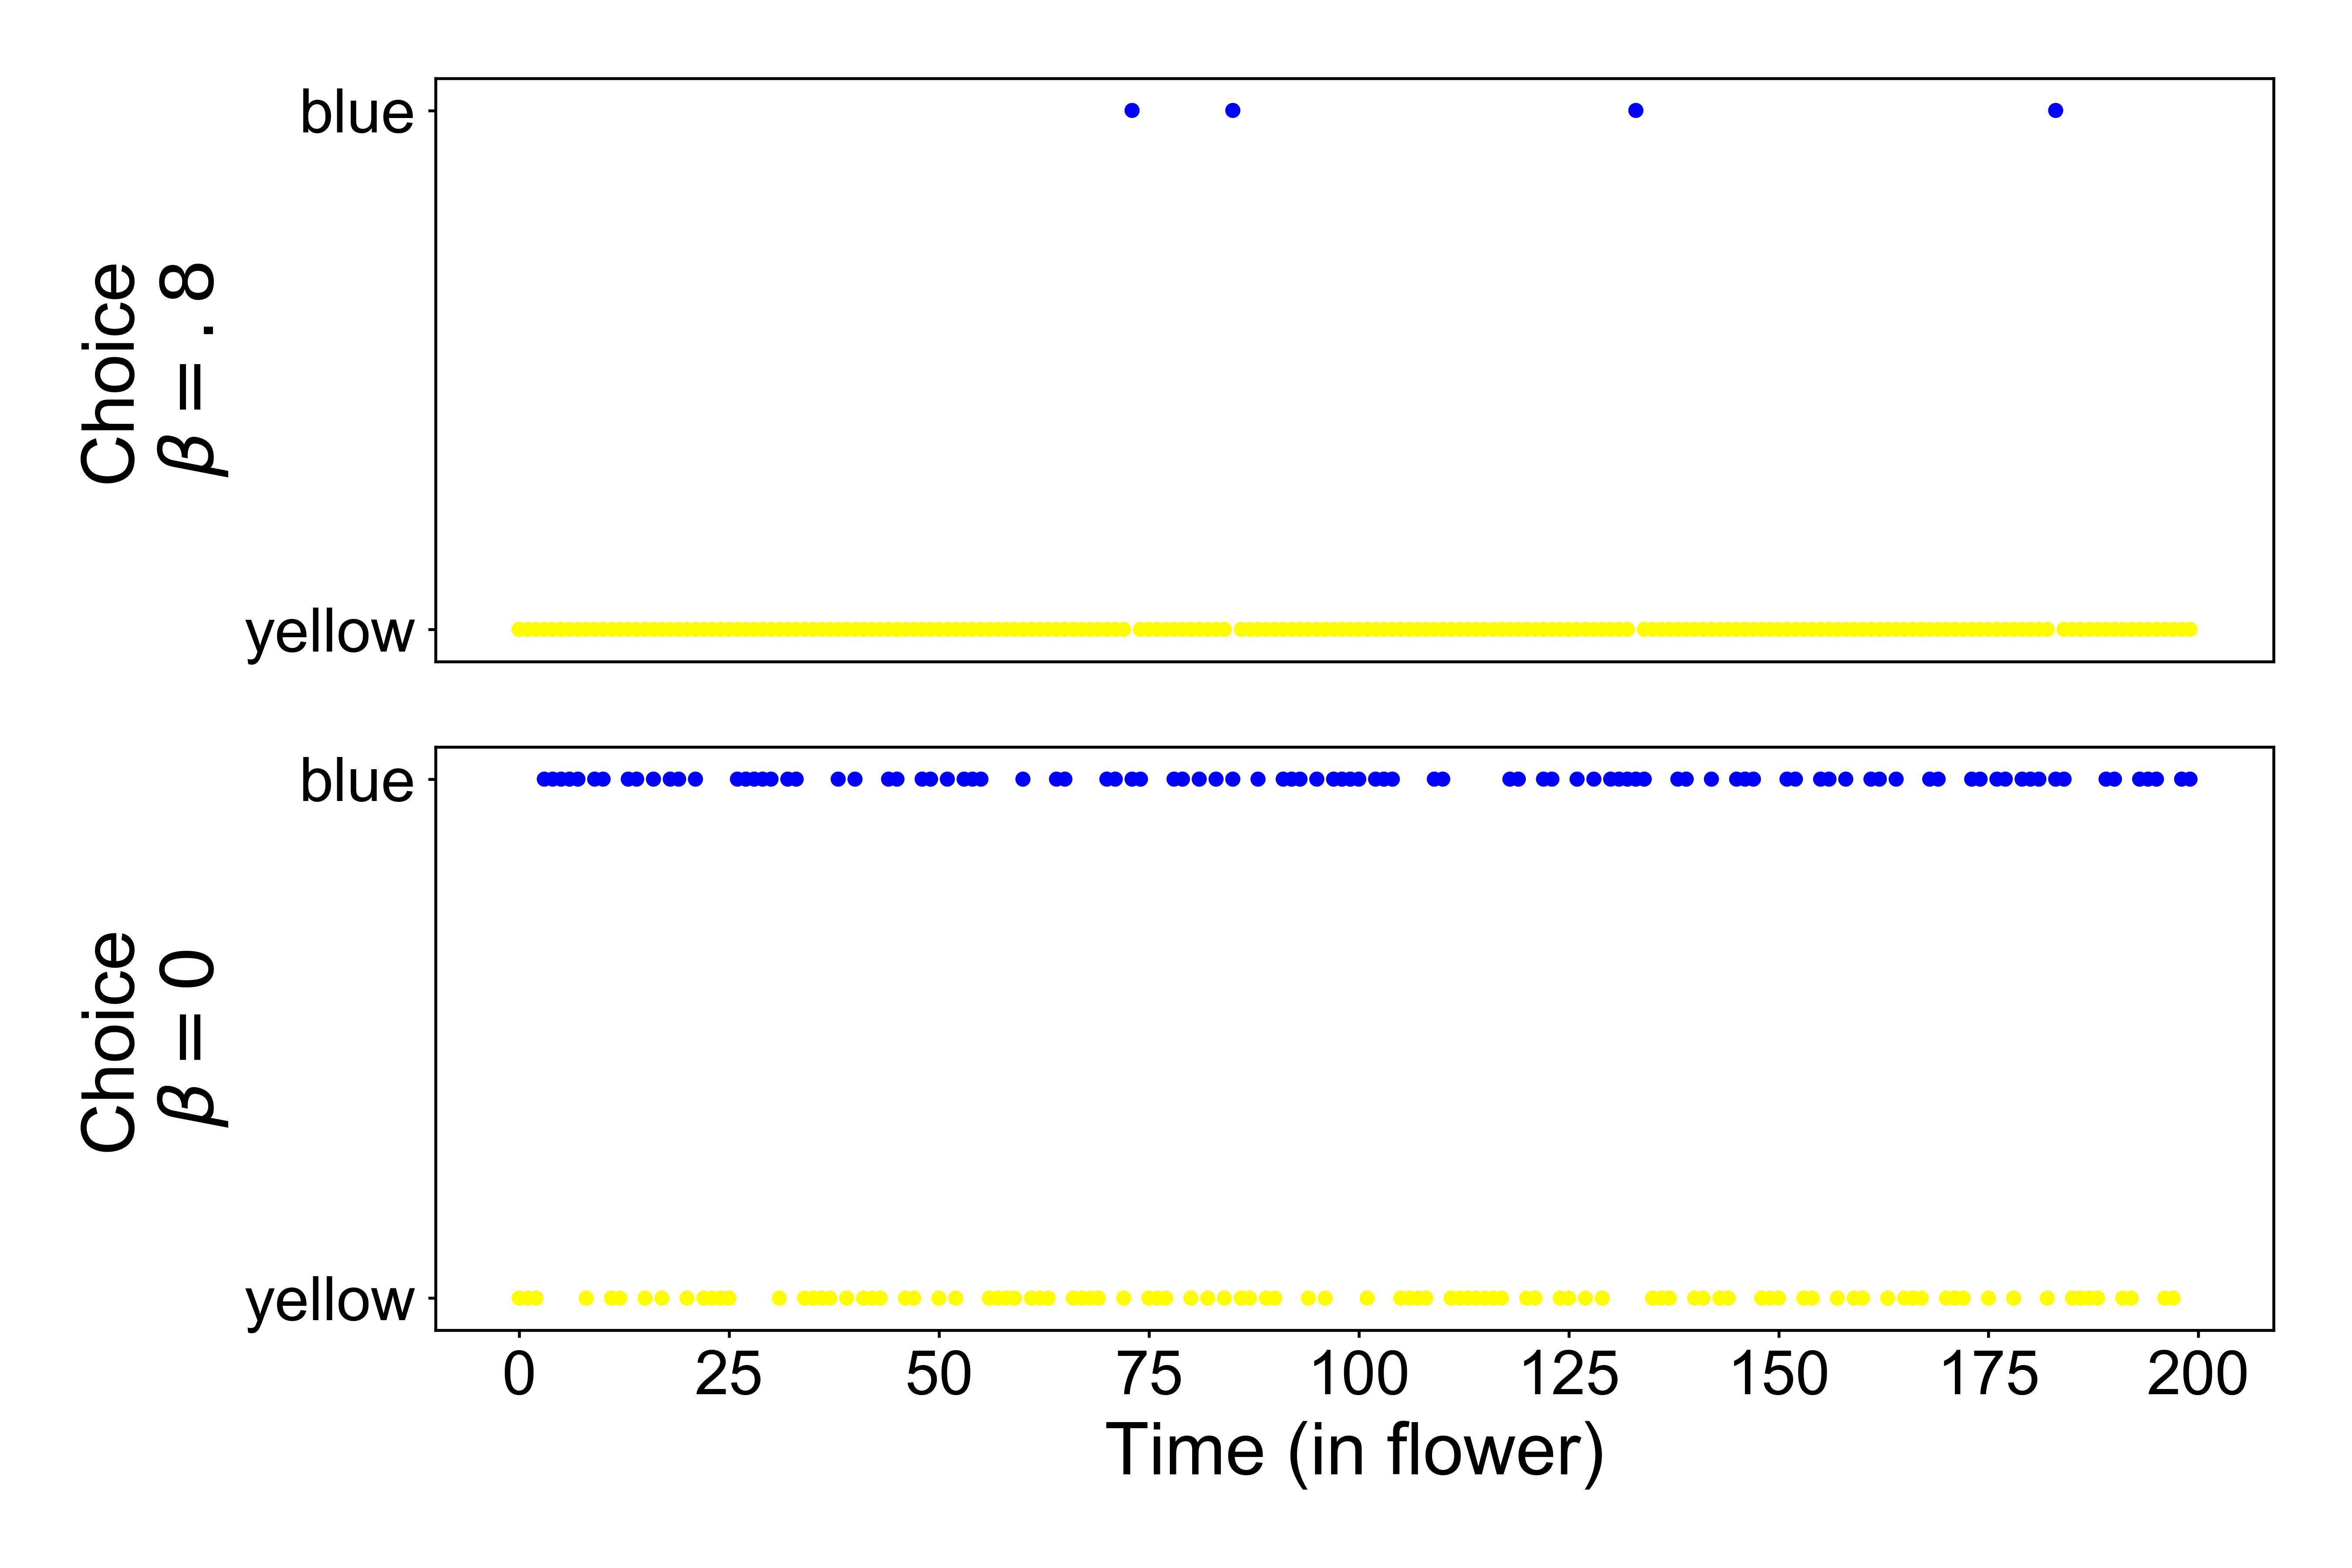
\includegraphics[width=.8\linewidth]{fig2_report11.png}
\caption[growing population]{Probability of choosing a blue flower, depending on the difference between the internal estimates of blue and yellow flowers, and on the $\beta$ parameter.}\label{fig:fig8}
\end{figure}

Let us now combine delta-rule and the softmax-policy: in a changing environment, the agent needs to keep learning the contingencies between stimulus and reward. Let's say the blue flowers yield a reward of $8$ and the yellow ones of $2$ the first day (the 100 first flowers), and the opposite pattern for the second day (the 100 next flowers). To complexify, let's say the initial estimates of the flowers' return are $m_b = 0$ and $m_y = 5$. Figure \ref{fig:fig9} shows what could happen: first, as the difference between the internal estimates $d$ is high in favor of the yellow flowers, the probability of choosing a blue one (and of learning its real value of 8) is low. However, as $m_y$ decreases from 5 to its real value 2, the probability of choosing a blue flower increases, and when it happens, $m_b$ grows rapidly, and soon the choices are dominated by blue flowers. The same thing happens the second day when the rewards changes.\\

\indent If we had $\beta = 0$, the choice would be random, independent of the estimates. In such a case, the agent always ``explore" its options, and so detects changes in the enviroment more rapidly. However, contrary to the agent in Figure \ref{fig:fig9} who ``exploited" the higher return flower and sometimes explored, the cumulative reward would be around 1000 ($200*(2+8)/2$), whereas the above-mentioned agent obtained 40\% more.

\begin{figure}[H]
\centering
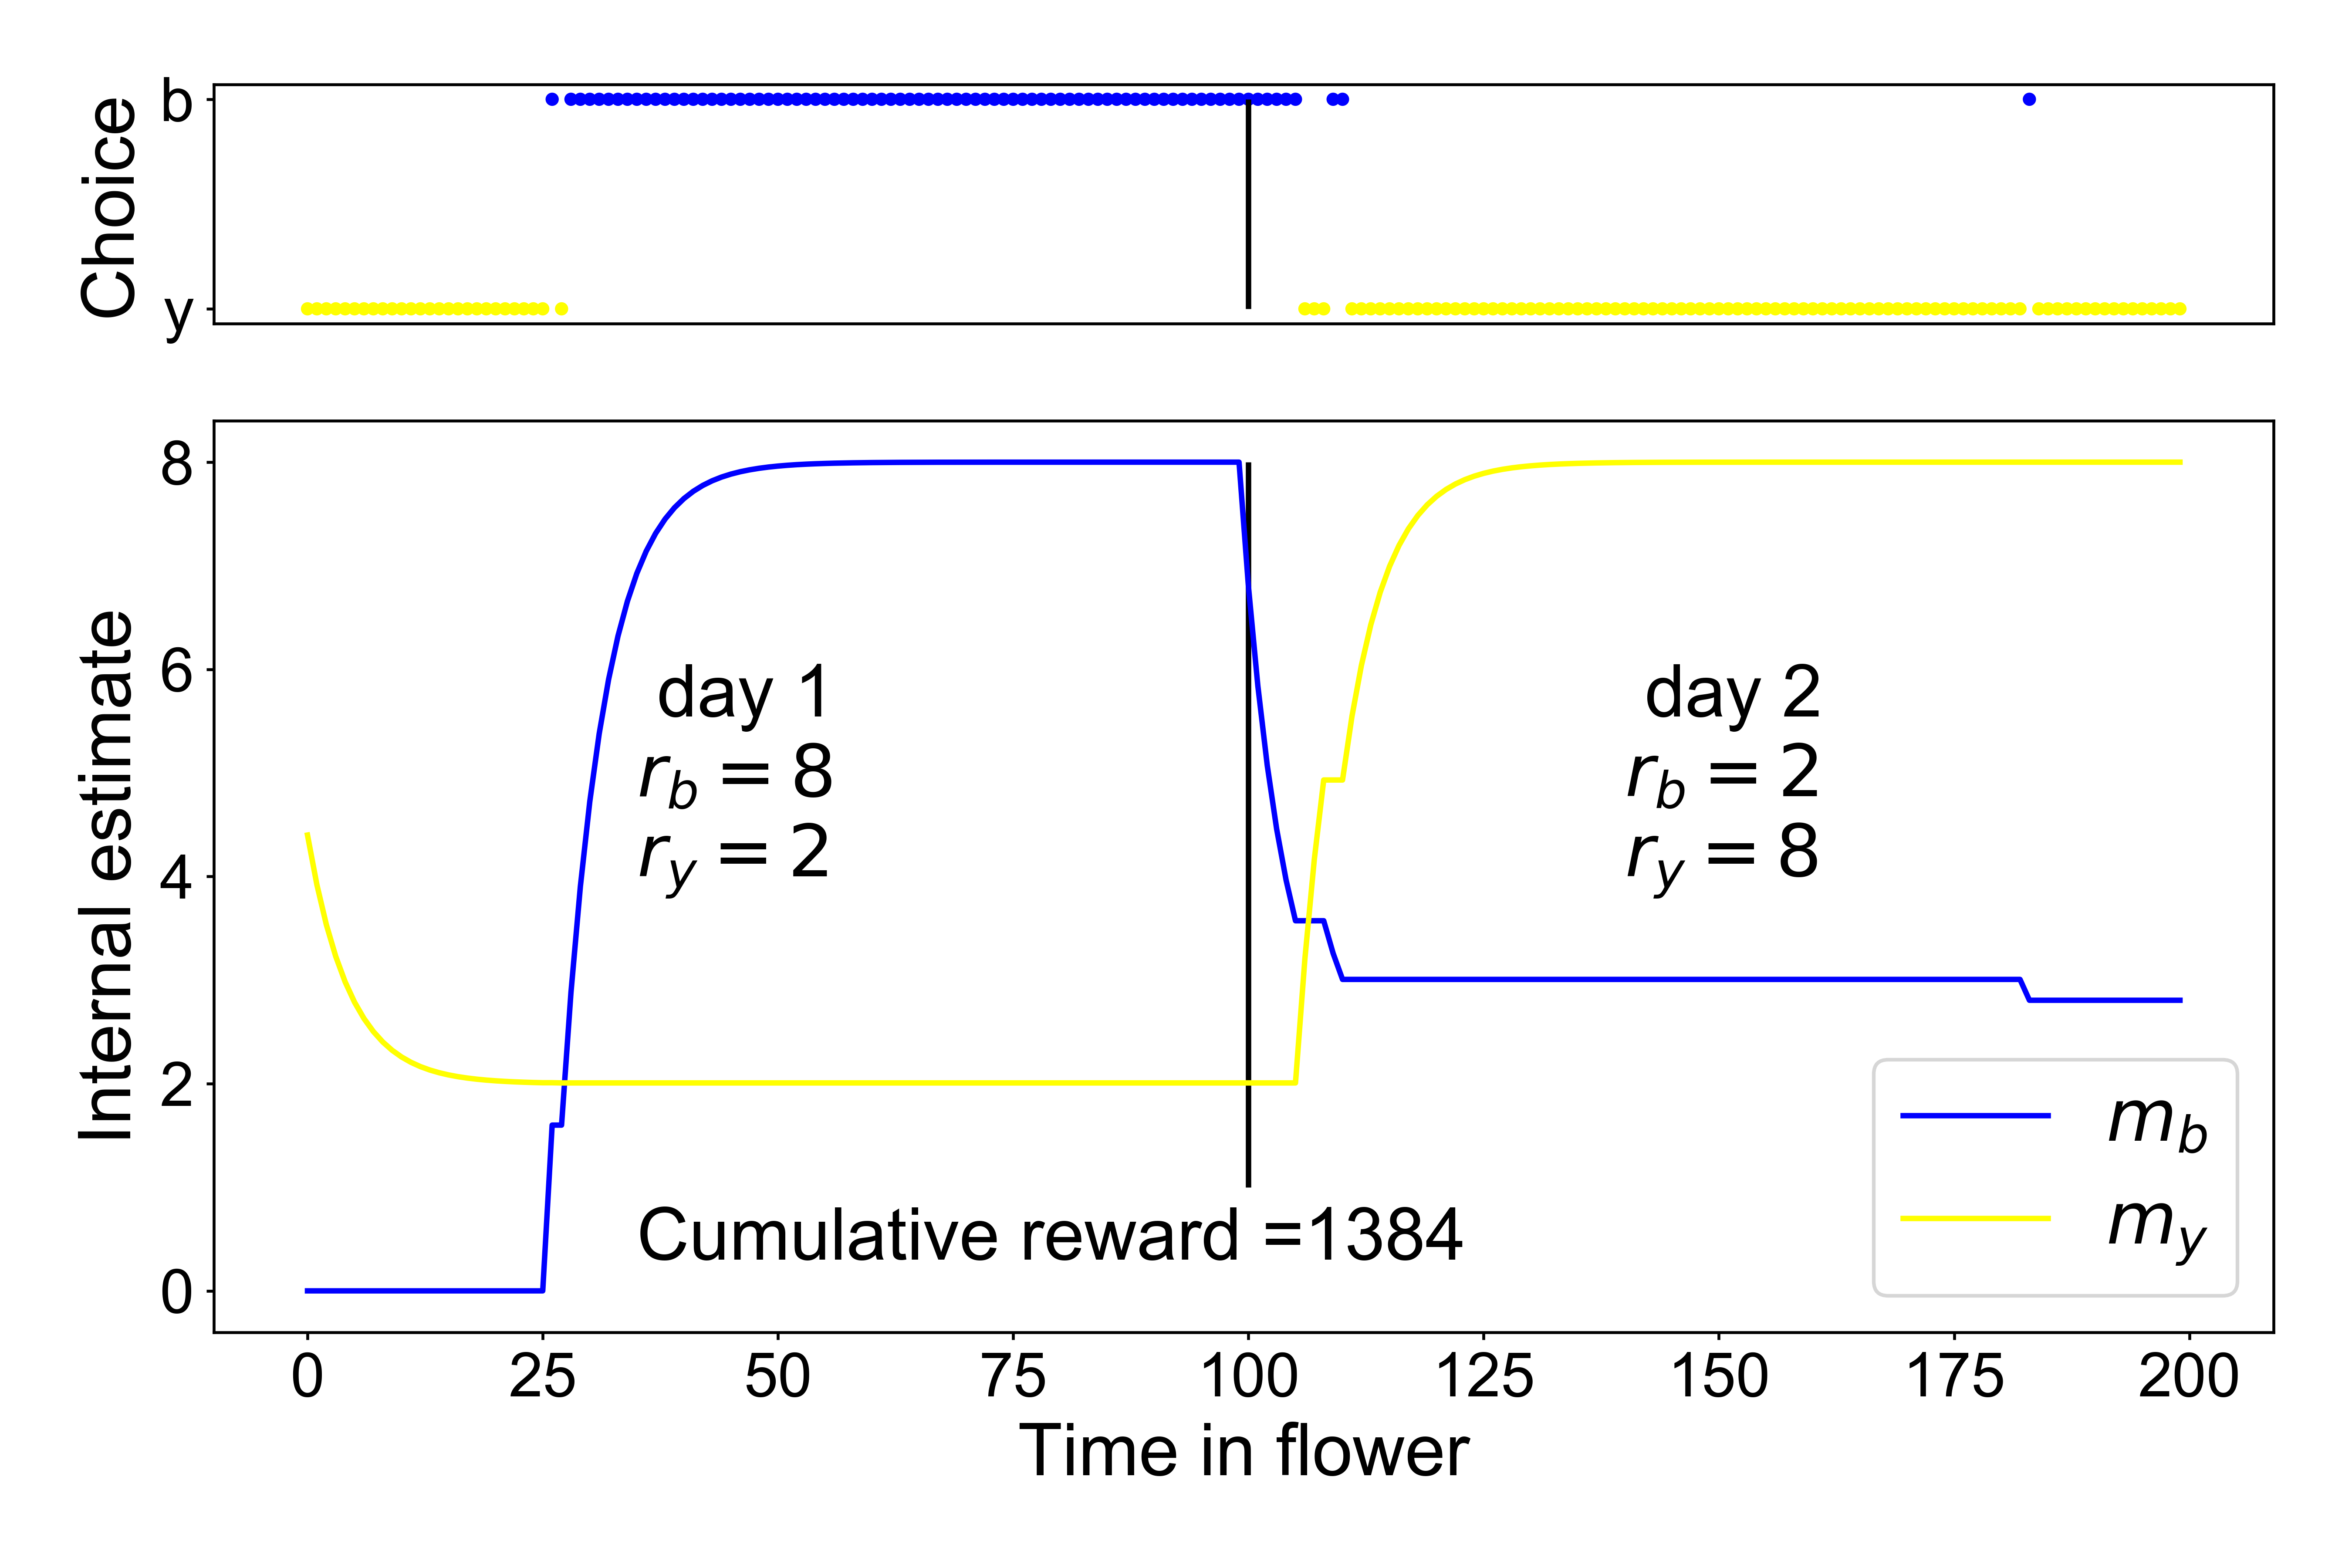
\includegraphics[width=.8\linewidth]{fig2_report12.png}
\caption[growing population]{Up. Choice of either blue or yellow flower in the two days. Down. Internal estimates $m_b$ and $m_y$ through time, in the changing environment described above. The temperature parameter $\beta = 1$ and the learning rate is $\epsilon = .2$}\label{fig:fig9}
\end{figure}
 %----------------------------------------------------------------------------------------
 %	SECTION 3
 %----------------------------------------------------------------------------------------
 \subsection{Drift diffusion model and evidence accumulation}

\indent\indent Another way to consider decision is as a dynamic process through time. This holds especially true for perceptual decision making, where one needs to \textit{accumulate evidence} from one's percepts in order to form an opinion, especially when there is little coherence in the stimulus we are attending. For instance, many neuroscientific experiments use random dot motion tasks (or 2 alternative forced-choice tasks; 2AFC), in which the stimulus is dozens of dots moving in different directions at the same time, and the subject must determine which direction is the more present direction.
\\
\indent One model of decision in such situation is the drift diffusion model (DDM), and it actually fits behavior as well as neuronal activity in some parts of the brain (Gold \& Shalden 2007). In simple terms, it postulates that a new internal estimate $x$ evolves in time through \textit{sequential sampling} of the difference between direction estimates. When the estimate $x$ reaches a threshold $\mu$ or $-\mu$, a decision is made in favor of one direction.
\\ \\
\indent This model is particularly prominent in the field, because it fits perfectly to neurons' firing rates in specific brain areas. First, the medial temporal area of the occipital (visual) cortex (MT) neurons have firing rates correlated with coherence of the motion towards a specific direction, that can be dubbed as \textit{evidence representation}. More interestingly, other regions like the laterial intra-parietal area (LIP) have an \textit{evidence accumulation} behavior. Specifically, their firing rate increases as a function of the MT signal (through sequential sampling). And when LIP neurons firing rate reaches a threshold $\mu$, an observable decision is made.
\\
\indent Furthermore, there are different sensitivities in MT neurons, such that some are specific to a single direction. We can simplify the problem by looking at 2 MT neurons' firing rates $m_A$ and $m_B$, respectively sensitive to motion in direction $A$ and $B$, in a 2AFC task. The firing rate of an evidence accumulating neuron in LIP can thus be formalized as integrating the difference between $m_A$ and $m_B$ over time:

\begin{align*}
\dot{x} = m_A - m_B + \sigma \eta(t)
\end{align*}

\noindent where $\eta(t)$ is a noise term, as the firing rate of neurons is noisy, and the percept might not be exactly stable in time as our attention moves and oscillates. Then, if $x$ reaches $\mu$ a decision is made in favor of $A$; and in favor of $B$ if it reaches $-\mu$. This can be approximated numerically:

\begin{align*}
x(t + \Delta t) &= x(t) + \dot{x}\Delta t \\
                &= x(t) + (m_A - m_B)\Delta t + \sigma \eta(t) \sqrt{\Delta t} \;\;\;\;\;\;\; \text{(as this is a stochastic differential equation)}
\end{align*}

Let's assume $m_A$ and $m_B$ are stable over time, choose a stepwidth $\Delta t$, a noise level $\sigma$, and a gaussian noise $\eta(t)$. We can then visualize the evidence accumulating over time (Figure \ref{fig:fig10} Left). If we determine a threshold $\mu$ at which a decision is made, we can now simulate reaction times (Figure \ref{fig:fig10} Right). It should also be taken into account that there is an incompressible time when responding, comprising notably of perception and motor planning. \\
\indent Interestingly, Figure \ref{fig:fig10} shows that even with a small difference between $m_A$ and $m_B$, and a relatively low threshold (\textit{i.e.} the ``wrong" threshold is more likely to be reached), there is relatively few wrong trials (choice $B \approx 2\%$ of simulations) and late $B$ decisions seem even more scarce.


\begin{figure}[H]
\centering
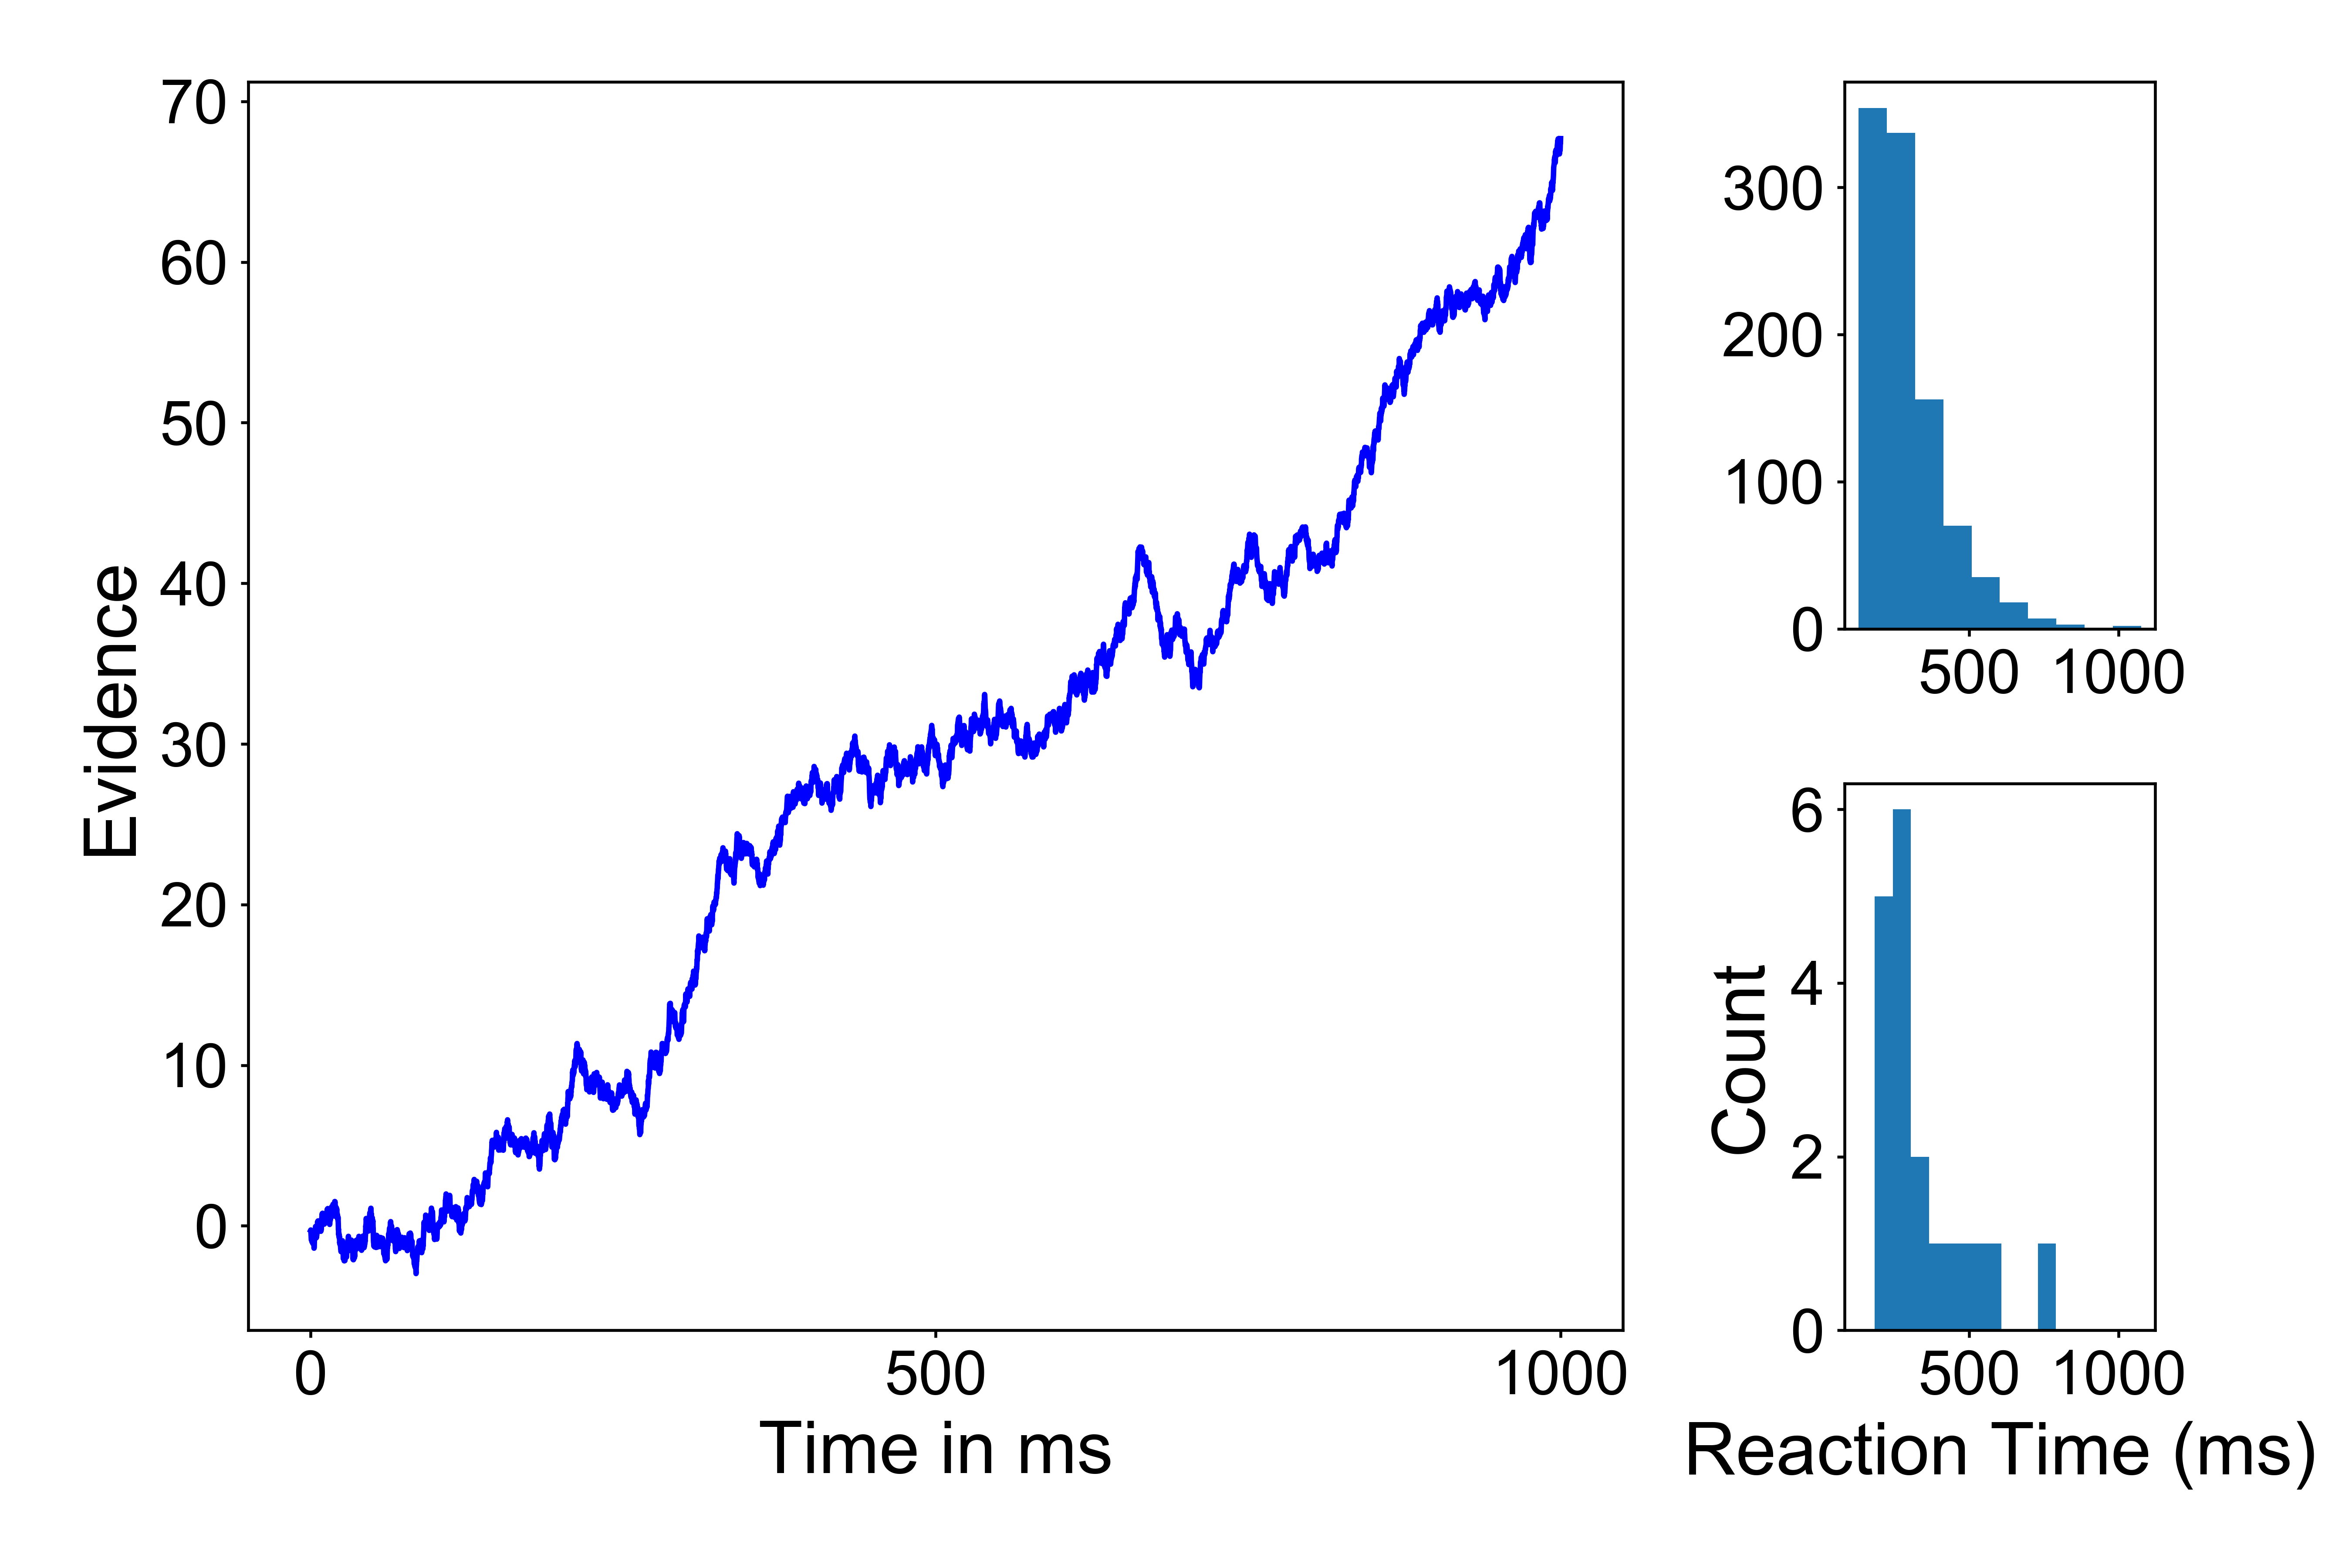
\includegraphics[width=.8\linewidth]{fig2_report13 (2).png}
\caption[growing population]{\textbf{Left.} Simulaion of evidence (arbitray units) accumulating through time for $m_A =1$, $m_B = .95$, $\Delta t = .1$ ms, $\sigma=.5$ and $\eta(t)$ is a random number following a normal distribution of mean 0 and variance 1. \textbf{Right.} Reaction times (RT) distribution for choice $A$ (Up) and $B$ (Down) for 10000 iterations of the simulation, with 100ms of incompressible processing added, for $\mu=10$.}\label{fig:fig10}
\end{figure}

Moreover, the speed of the accumulation depends on the signal to noise ratio, but obviously also on the amplitude of the difference $m_e$ between $m_A$ and $m_B$. Figure \ref{fig:fig11} (left) shows indeed steeper curves for higher $|m_e|$ values. \\
\indent This model is pretty reliable and acually fits a lot of neural (firing rate of neurons of different functionnal areas) and behavioral data (choice and reaction time). In contrast, the softmax policy model only explains choice probability, and can not account as well for neural and behavioral variability.

\begin{figure}[H]
\centering
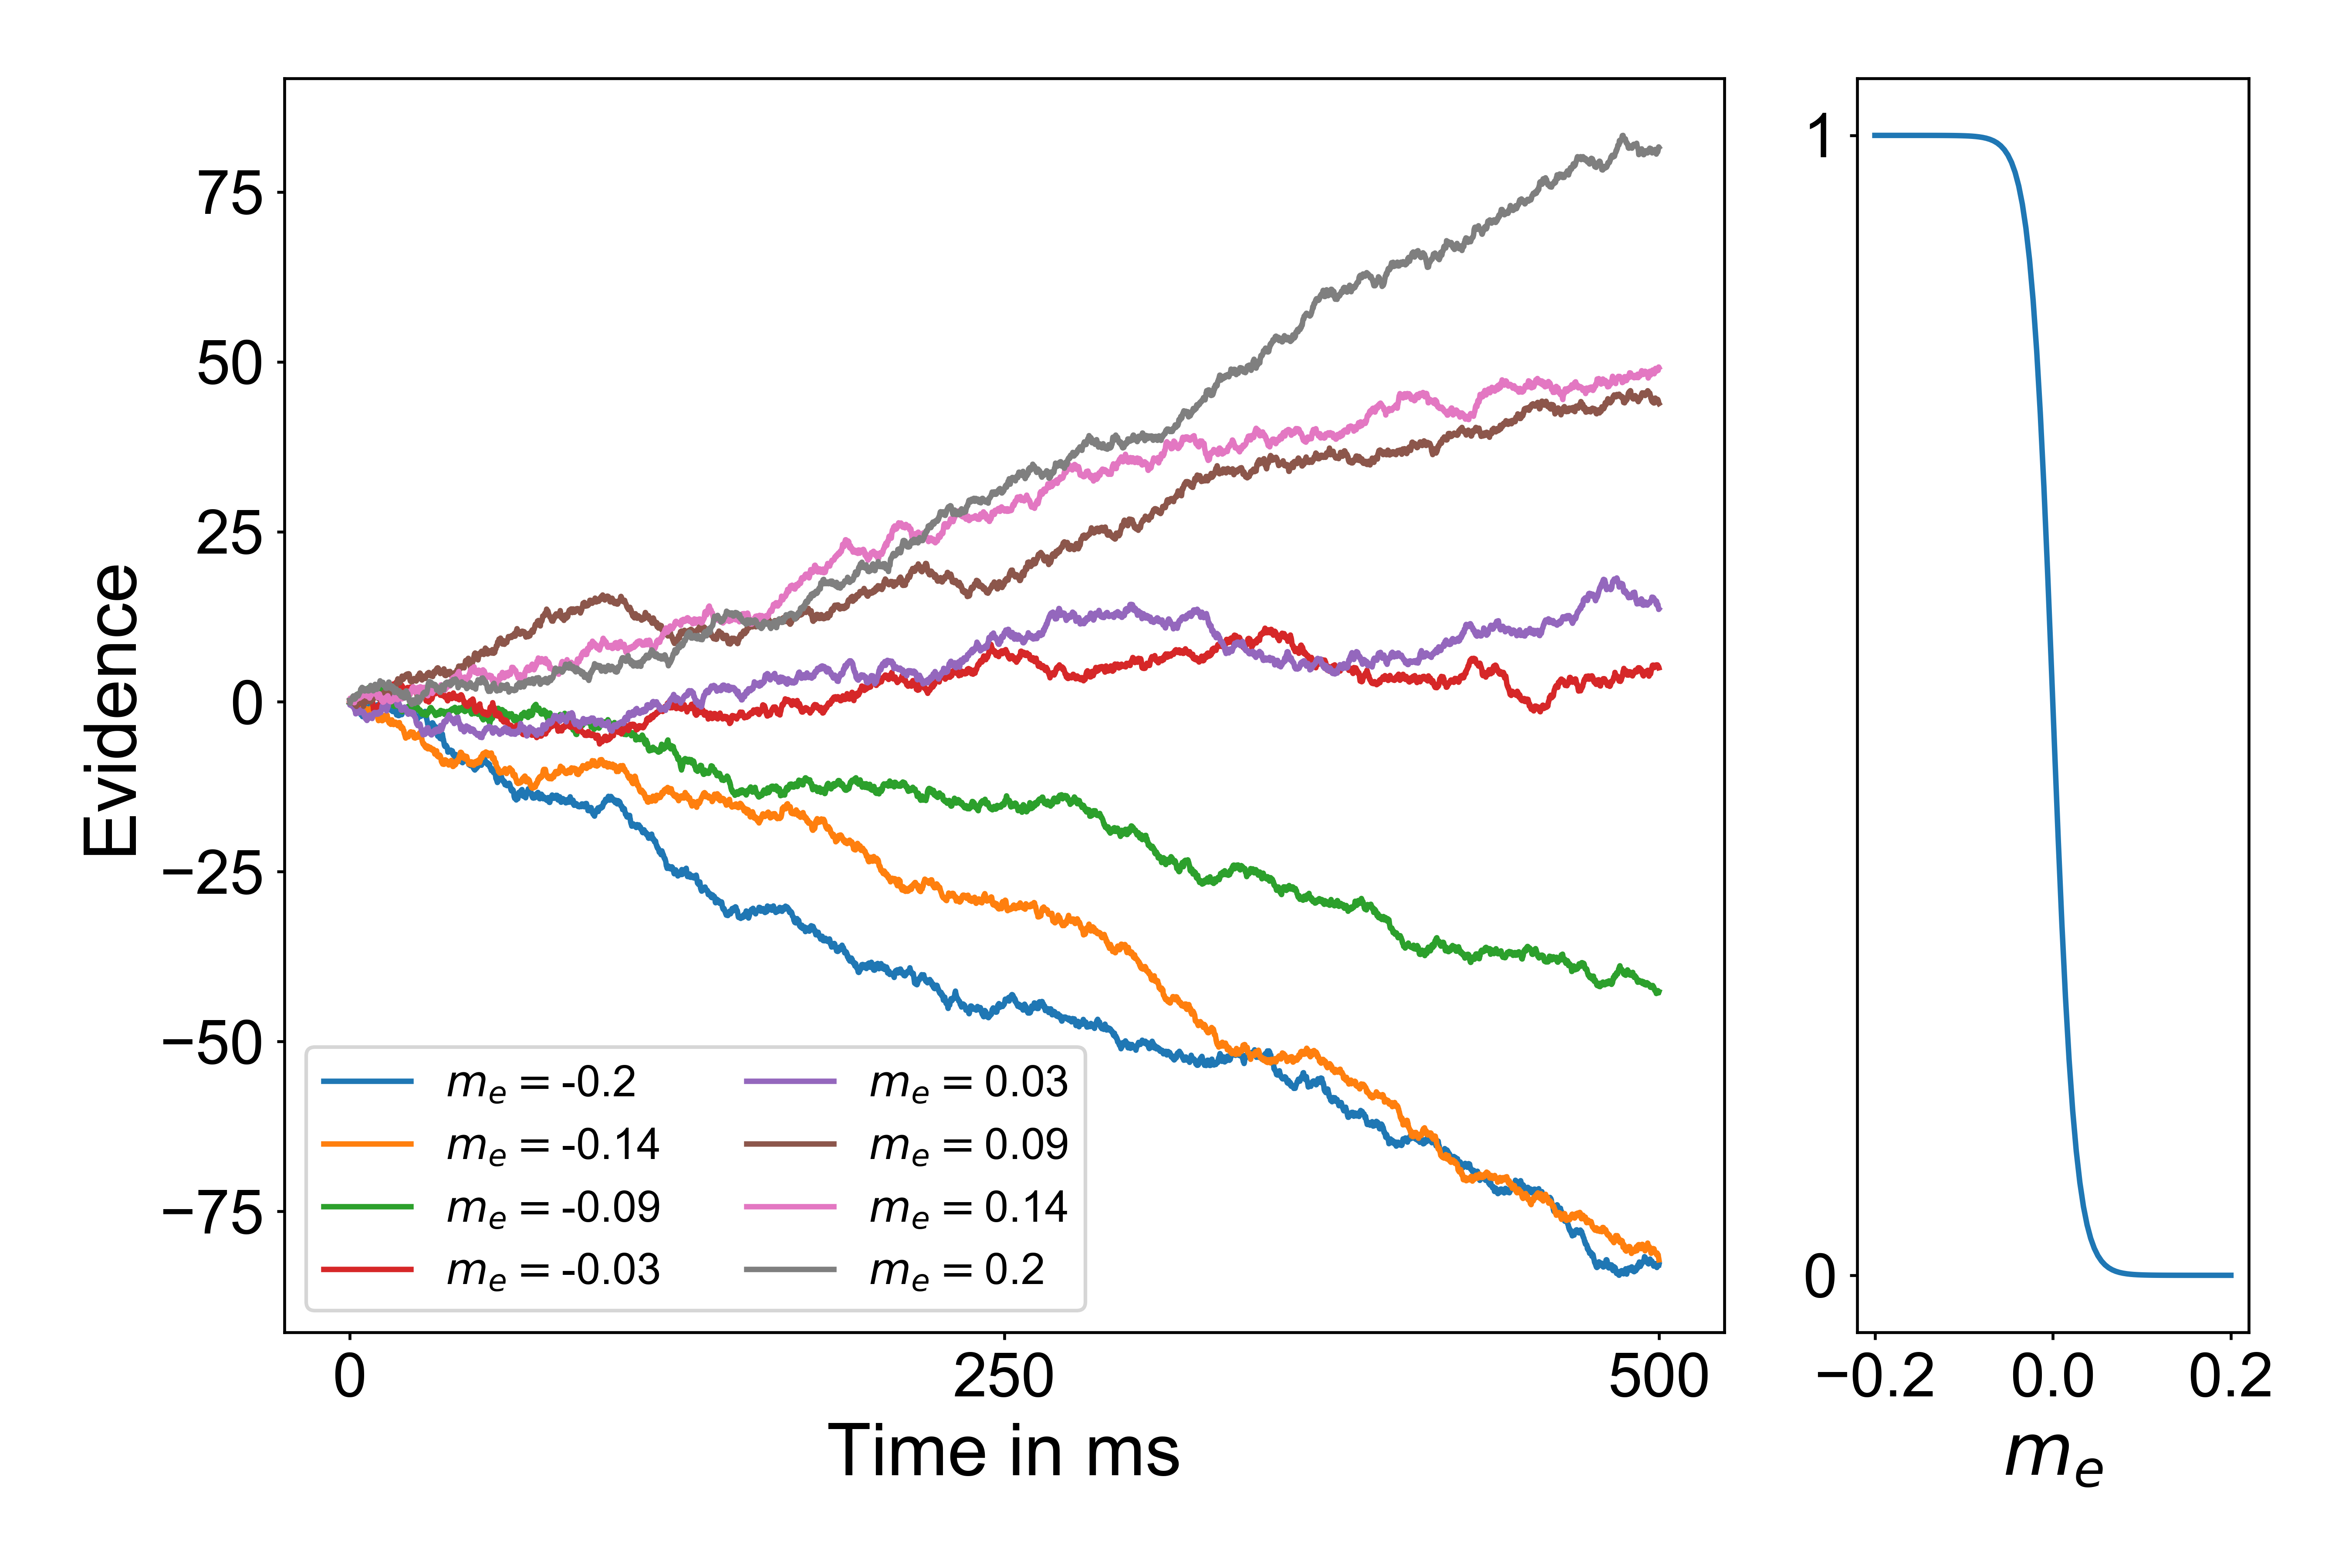
\includegraphics[width=.8\linewidth]{fig2_report14.png}
\caption[growing population]{\textbf{Left.} Simulation of evidence accumulation for difference values of $m_e$. Other parameters same as figure \ref{fig:fig10}. \textbf{Right.} Probability of $B$ choices as a function of $m_e$ given the softmax policy. Parameter $\beta=2\mu / \sigma^2 = 80$. }\label{fig:fig11}
\end{figure}

%----------------------------------------------------------------------------------------
%	Conclusion
%----------------------------------------------------------------------------------------
\section{Conclusion}
\indent The models described in this report can have many applications. For instance, they can be used to try to predict behavior (e.g. by economists), without assuming that it really is how it is implemented in the brain. But they can also help us understand how our mind - and our brain - works, as we can observe that the parameters of models fitted to behavioral data are actually correlated to neural activity, for instance observed with fMRI (Lebreton et al. 2012). Those models can indeed sometimes explain up to the firing rate of specific neurons, and help us uncover the mind at the computational, algorithmic and implementation level.


\end{document}
